% This is samplepaper.tex, a sample chapter demonstrating the
% LLNCS macro package for Springer Computer Science proceedings;
% Version 2.20 of 2017/10/04
%
\documentclass[runningheads]{llncs}
%
\usepackage{graphicx,url}
\usepackage[utf8]{inputenc}
\usepackage[american]{babel}
\usepackage{booktabs}
\usepackage{indentfirst}
\sloppy

\usepackage{cite}
\usepackage{amsmath,amssymb,amsfonts}
\usepackage{algorithmic}
\usepackage{graphicx}
\usepackage{textcomp}
\usepackage[flushleft]{threeparttable}
\usepackage{longtable}
\usepackage{array}
\newcolumntype{P}[1]{>{\centering\arraybackslash}p{#1}}
\usepackage{graphicx}
\usepackage{listings}
\usepackage{todonotes}
\usepackage[inline]{enumitem}
\usepackage[draft]{hyperref}
\usepackage{multicol}

\newcommand{\footlabel}[2]{%
    \addtocounter{footnote}{1}%
    \footnotetext[\thefootnote]{%
        \addtocounter{footnote}{-1}%
        \refstepcounter{footnote}\label{#1}%
        #2%
    }%
    $^{\ref{#1}}$%
}
\newcommand{\footref}[1]{%
    $^{\ref{#1}}$%
}


% Used for displaying a sample figure. If possible, figure files should
% be included in EPS format.
%
% If you use the hyperref package, please uncomment the following line
% to display URLs in blue roman font according to Springer's eBook style:
% \renewcommand\UrlFont{\color{blue}\rmfamily}

\begin{document}
%
\title{A platform to analyse impacts of the exception events on the bus velocity of São Paulo\thanks{This research is part of the INCT of the Future Internet for Smart Cities funded by CNPq, proc. 465446/2014-0, CAPES proc.88887.136422/2017-00, and FAPESP, proc. 2014/50937-1.}}
%
%\titlerunning{Abbreviated paper title}
% If the paper title is too long for the running head, you can set
% an abbreviated paper title here
%
%\author{Felipe Cordeiro Alves Dias\inst{1}\orcidID{0000-0003-4648-1498} \and
%Daniel Cordeiro\inst{1}\orcidID{0000-0003-4971-7355} \and
%Rodolfo da Silva Simões\inst{1}\orcidID{2222--3333-4444-5555}}

%\author{Felipe Cordeiro Alves Dias\inst{University of São Paulo}\orcidID{0000-0003-4648-1498} \and
%Daniel Cordeiro\inst{University of São Paulo}\orcidID{0000-0003-4971-7355} \and
%Rodolfo Simoes\inst{University of São Paulo}\orcidID{2222--3333-4444-5555}}
%
%\authorrunning{F.C.A Dias et al.}
% First names are abbreviated in the running head.
% If there are more than two authors, 'et al.' is used.
%
%\institute{University of São Paulo \\
%School of Arts, Sciences and Humanities \\ 
%\email{\{felipecavazotto, daniel.cordeiro, simoesrodolfo\}@usp.br}}
%
\maketitle              % typeset the header of the contribution
%
\begin{abstract}
%The abstract should briefly summarize the contents of the paper in
%150--250 words.

This work uses supervised learning to classify tweets in exception events, which are correlated with real data sources (AVL and GTFS) to understand the impacts of these events in the buses velocity of São Paulo.

\keywords{Smart cities \and social networks \and public transportation.}

\end{abstract}
%
%
%
%\section{First Section}
%\subsection{A Subsection Sample}
%Please note that the first paragraph of a section or subsection is
%not indented. The first paragraph that follows a table, figure,
%equation etc. does not need an indent, either.
%
%Subsequent paragraphs, however, are indented.
%
%\subsubsection{Sample Heading (Third Level)} Only two levels of
%headings should be numbered. Lower level headings remain unnumbered;
%they are formatted as run-in headings.

%\paragraph{Sample Heading (Fourth Level)}
%The contribution should contain no more than four levels of
%headings. Table~\ref{tab1} gives a summary of all heading levels.

%\begin{table}
%\caption{Table captions should be placed above the
%tables.}\label{tab1}
%\begin{tabular}{|l|l|l|}
%\hline
%Heading level &  Example & Font size and style\\
%\hline
%Title (centered) &  {\Large\bfseries Lecture Notes} & 14 point, bold\\
%1st-level heading &  {\large\bfseries 1 Introduction} & 12 point, bold\\
%2nd-level heading & {\bfseries 2.1 Printing Area} & 10 point, bold\\
%3rd-level heading & {\bfseries Run-in Heading in Bold.} Text follows & 10 point, bold\\
%4th-level heading & {\itshape Lowest Level Heading.} Text follows & 10 point, italic\\
%\hline
%\end{tabular}
%\end{table}


%\noindent Displayed equations are centered and set on a separate
%line.
%\begin{equation}
%x + y = z
%\end{equation}
%Please try to avoid rasterized images for line-art diagrams and
%schemas. Whenever possible, use vector graphics instead (see
%Fig.~\ref{fig1}).

%\begin{figure}
%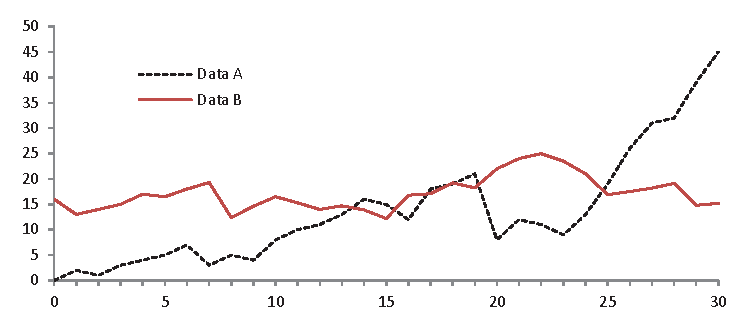
\includegraphics[width=\textwidth]{fig1.eps}
%\caption{A figure caption is always placed below the illustration.
%Please note that short captions are centered, while long ones are
%justified by the macro package automatically.} \label{fig1}
%\end{figure}
%
%\begin{theorem}
%This is a sample theorem. The run-in heading is set in bold, while
%the following text appears in italics. Definitions, lemmas,
%propositions, and corollaries are styled the same way.
%\end{theorem}
%
% the environments 'definition', 'lemma', 'proposition', 'corollary',
% 'remark', and 'example' are defined in the LLNCS documentclass as well.
%
%\begin{proof}
%Proofs, examples, and remarks have the initial word in italics,
%while the following text appears in normal font.
%\end{proof}
%For citations of references, we prefer the use of square brackets
%and consecutive numbers. Citations using labels or the author/year
%convention are also acceptable. The following bibliography provides
%a sample reference list with entries for journal
%articles~\cite{ref_article1}, an LNCS chapter~\cite{ref_lncs1}, a
%book~\cite{ref_book1}, proceedings without editors~\cite{ref_proc1},
%and a homepage~\cite{ref_url1}. Multiple citations are grouped
%\cite{ref_article1,ref_lncs1,ref_book1},
%\cite{ref_article1,ref_book1,ref_proc1,ref_url1}.
%
% ---- Bibliography ----
%
% BibTeX users should specify bibliography style 'splncs04'.
% References will then be sorted and formatted in the correct style.
%
% \bibliographystyle{splncs04}
% \bibliography{mybibliography}
%

\section{Introduction}

%In São Paulo 10\% of population lives in the Expanded Center area and 90\% in the Peripheral Belt~\cite{SA201722}, which characterizes an urban segregation responsible for numerous problems related to urban mobility. Especially in segregated cities, 

Exception events happen sporadically or suddenly and are capable of generating significant delays or even unavailability of the operation of public transport. This type of events are reported by citizens and authorities in Social Networks, which can be used by Smart City systems. As an example, the public transport can benefit by integrating Social Networks content with the planning, management and operational activities of public transport, addressing their respective sociotechnical factors~\cite{kuflik2017automating}. In this work we present a new platform validated with real and heterogeneous data sources (\textit{tweets}, AVL --- Automatic Vehicle Location and GTFS\footnote{\label{googleTransit}Google Transit: \url{https://developers.google.com/transit}. Accessed in December 11, 2018.} --- Google Transit Feed Specification data) to understand exception events impacts in the São Paulo' buses velocity.
%, affecting socioeconomically the citizens who need to get around by public transport to specific regions of the cities to carry out work activities, study, leisure, among others. 
%Exception events are .

%The platform allows to classify \textit{tweets} in exception events and automatic identification of which lines were affected, estimating their velocity reduction. To achieve this objective we (I) trained several models to classify exception events reported by the selected profiles, (II) developed a process to addresses extraction and geolocalization based on \textit{tweets}, which are (III) correlated with SPTrans's (responsible for the bus lines of the municipality of São Paulo) GTFS (commonly used to describe public transport data) data to find bus lines impacted by exception events in the São Paulo city and with (IV) AVL data to velocity impact characterization. Using this platform we characterized 60,984 events and found 10,027 exception events that impacted 1,073 bus lines. Besides, we found that social events have an average of 87,04\% impact on the average speedy of bus lines affected by a radius of 1,000m; urban events 70,11\%; accidents 66,51\% and natural disasters 59,77\%.

\section{Related Work}
\label{relatedWorks}
%According to a literature review, we found works that use \textit{tweets} processing to mitigation of problems related to public transportation. The reviewed studies can be classified in \emph{event impact analysis}, \emph{planning} and \emph{management of public transportation}. For example, \cite{Wen2016} used \textit{tweets} to analyze the impact of the terrorist attacks in Paris (2015) on mobility patterns regarding the use of public transport. Similarly, \cite{Itoh2016} developed a tool based on \textit{tweets} to visualize and explore the decisions of passengers of the Tokyo Metro before abnormal events such as typhoons, fires, earthquakes, etc. In this same context, \cite{Ni2016} proposed a technique to predict passenger flow in the New York Metro and identify events based on \textit{hashtags}. Whereas in \cite{Chen2016} the relationship between traffic events and the demand for bicycles was analyzed.
%
Several works studies how to use \textit{tweets} processing for analyzing problems related to public transport. These studies can be classified into \emph{event impact analysis}, \emph{planning} and \emph{management of public transport}. For example, \cite{Wen2016} used \textit{tweets} to analyze the impact of the terrorist attacks in Paris (2015) on mobility patterns regarding the use of public transport. Similarly, \cite{Itoh2016} developed a tool based on \textit{tweets} to visualize and explore the decisions of passengers of the Tokyo Metro in abnormal events such as typhoons, fires, earthquakes, etc. In this same context, \cite{Ni2016} proposed a technique to predict passenger flow in the New York Metro and identify events based on \textit{hashtags}. \cite{Chen2016} studied the relationship between traffic events and the demand for bicycles.

In respect to public transport planning and management, \cite{Mukherjee2015} presents a platform developed and used by the Bangalore Public Transport Agency, which allows report issues related to public transport, improving the operation planning and the service provided to the population. Analogously, \cite{Gutev2016} used \textit{tweets} to identify the popularity of points of interest and age distribution, in order to determine the best points for bicycle stations and thus encourage the use of this mode of transport. Also related to the points of interest, \cite{Maghrebi2015} used \textit{tweets} to identify human activities patterns and their respective impacts on the demand for public transport.

In \cite{Gal-Tzur2014} a hierarchical approach was created to classify \textit{tweets} related to transport. They have demonstrated that it is possible to use this information for transportation planning and management purposes. This technique was applied in a case study associated with sporting events in the United Kingdom. The hierarchy is composed of three levels (I) \textit{tweets} classified among those that express the need for transport services, opinions and incidents; (II) identification of the transport category and (III) topics.

Another study that contributes to the planning of public transport is the one carried out in \cite {Gkiotsalitis2015, Gkiotsalitis2016}, in which \textit{tweets} were processed to identify user disposition to trips related to leisure, suggesting to them activities with less time of travel and probability of delays. Another relevant point considered was the level of access to public transport, which, when high, positively impacts people's happiness and correlates with positive feelings, according to the analysis of feelings carried out by \cite{Guo2016}, using \textit{tweets} published in Greater London.

Neither of the presented works tackle the identification of different types of exception events from \textit{tweets} published by an authority to characterize the velocity impact on buses of São Paulo. In this work we propose a new platform, explained ahead, for deal with this problem.
%that deal with: 
%(I) training a model to classify exception events published by authority profiles, (II) address extraction from semi-structured \textit{tweets} (since \textit{tweets} from authorities uses a formal language with specific patterns \cite{Gal-Tzur2014}) using a \textit{Regex} pattern; (III) finding bus lines and addresses impacted by exception events in the São Paulo city through \textit{tweets} and GTFS data and (IV) impact characterization. 
The cited works are connected to our on aspects related to \textit{tweets} processing for analysis of the impact of events on public transport, planning and management.

%\section{Basic concepts}

%\subsection{Social Networks}
%\label{sns}
%
%Social Networks (SN) can be defined as networks that have many relationships, with large connected components, clustering coefficients and degree of reciprocity. Such features, e.g, are found on \textit{Facebook}\footnote{\url{https://www.facebook.com}. Accessed in December 09, 2018.}. Another SN is  \textit {Twitter}\footnote{\url{https://twitter.com}. Access in December 09, 2018.}, which besides having the social networking features mentioned can also be characterized as an Information Network. In this type of network the dominant interaction is the dissemination of information between relationships, with low reciprocity index \cite{myers2014information}.
%
%On \textit{Twitter} the information (\textit{tweets}) is published containing a maximum of 280 characters; each publication can receive \textit {retweets} (to be shared by other users), comments (directly in the \textit{tweet} --- \textit {replies} --- or privately via the message box) and \textit{likes} (indicator of how many users liked the post), in addition to these features, \textit{tweets} may contain mentions to other users (@\textit{profile}) and labels (\#\textit{hashtag}) indicating subjects, categories, etc. Due to the characteristics mentioned previously, the \textit {Twitter} has been an important social network for sharing information and everyday events. Such events can be classified as social events, capable of describing from routine events to crisis situations (natural disasters, social mobilizations, among others) \cite{zhou2014event, atefeh2015survey}.

%\subsection{Smart Cities and Public Transport}
%\label{smartCities}
%
%The concept of Smart Cities (SC) has been defined mainly as sustainable and socially inclusive cities~\cite{Wang2017}, which use Information and Communication Technologies (ICTs) to efficiently manage natural resources, energy, transportation, waste, etc.~\cite{Ahvenniemi2017}. ICTs permeates urban systems and physical spaces, which has been accentuated by the increasing number of sensors and devices connected to the Internet of Things (IoT); voluntary data and existing content on SN about daily events. Such heterogeneous sources generate large amounts of data, used to develop SC services \cite{Finger2017, Ang2017}.
%
%The development of SC services has challenges related to connectivity (network infrastructure, interoperability and standards, power consumption and scalability) and related to data (capacity and location of data storage, extraction, processing, analysis, integration and aggregation). Besides, data analysis has issues related to correlation, inference of data from different domains, machine learning, real-time processing, and new-use proposals for data from existing infrastructures \cite{Ang2017, Xiao2017}.
%
%In the public transport context, the GTFS is a specification of a common format to exchange static information on public transport. A feed specified in static GTFS consists of text files. In this research we correlate SPTrans's static GTFS and AVL data with \textit{tweets} from the selected accounts.

%Different properties of a public transport network --- properties like stops, routes, journeys, and other time-related data --- are defined on \textit{Google Transit} on different files, as follows:

%\begin{enumerate*}
%\item \textit{agency.txt}\footnote{\label{note1}GTFS required files.}--- Contains one or more public transport agencies as data source.
%\item \textit{stops.txt}\footnoteref{note1}--- Contains the individual places where vehicles pick up or drop off passengers.
%\item \textit{routes.txt}\footnoteref{note1}--- Contains the routes of a travel group displayed to passengers as a single service.
%\item \textit{trips.txt}\footnoteref{note1}--- Contains the trips for each route. A trip is a sequence of two or more stops that occurs at a specific time.
%\item \textit{stop\_times.txt}\footnoteref{note1}--- Contains the departure and arrival times of vehicles at specific stops for each trip.
%\item \textit{calendar.txt}\footnoteref{note1}--- Contains dates for service IDs that use a weekly schedule. They specify when the service begins and ends, as well when the service is available.
%\item \textit{calendar\_dates.txt}\footnoteref{note2} --- Contains the exceptions for service IDs defined in the \textit{calendar.txt} file. If the \textit{calendar\_dates.txt} file includes \textit{all} service dates, it can be specified in the place of \textit{calendar.txt}.
%\item fare\_attributes.txt (optional) --- Contains information about the fares of the routes of a public transport company.
%\item \textit{fare\_rules.txt}\footnote{\label{note2}GTFS optional files.}--- Contains rules for the implementation of fare information for the routes of a public transport company.
%\item \textit{shapes.txt} (optional) --- Contains rules for drawing lines on a map to represent the paths of a public transport company.
%\item \textit{frequencies.txt}\footnoteref{note2}--- Contains the intervals between trips on the routes.
%\item \textit{transfers.txt}\footnoteref{note2}--- Contains rules for connections at transfer points between paths.
%\item \textit{feed\_info.txt}\footnoteref{note2}--- Contains additional information about the \textit{feed}, including editor, version, and validity information. \\
%\end{enumerate*}

%In addition to the static GTFS exists the realtime GTFS, which is a static GTFS extension. To use real-time feeds it is necessary to define the static files of GTFS, which are used in GTFS realtime to obtain the information of the public transport system. GTFS realtime is not part of the scope of this article, but the specification can be found in Google Transit. 

%\begin {enumerate*}
%\item Low level (common problems to NLP).
%\begin{enumerate*}
%\item \textit{Sentence boundary disambiguation} (SBD): processing utilized to identify the beginning and ending of a sentence.
%\item \textit{Tokenization}: processing utilized to obtain the words existing in a sentence, includes the removal of numbers, punctuations and characters that do not belong to the alphabet.
%\item \textit{Part-of-speech tagging}: processing utilized to identify the grammatical classifications (verb, subject, adjective, etc.) of the words in a sentence, considering their respective meanings and context in which they are inserted.
%\item \textit{Morphological decomposition}: processing utilized for morphological decomposition of a given word into its inflected form using lemmatization (word lemma identification) or stemming (identification of the root of the word using heuristics to determine the location of its flexion).
%\item \textit{Shallow parsing} (chunking): processing utilized for identifying segments of a sentence, such as verbal and nominal phrases, etc., based on \textit{tokens} that constitute the part-of-speech.
%\end{enumerate*}

%\item High level (application of NLP to specific problems, based on low level problem).
%\begin {enumerate*}
%\item \textit {Spelling / grammatical error identification and recovery}: iterative processing realized for identification and correction of grammatical and typing errors.
%\item \textit{Named Entity Recognition} (NER): processing realized for identification and categorization of specific words or phrases (entities).
%\item \textit{Word Sense Disambiguation} (WSD): processing to identify the meaning of a word in a sentence.
%\item \textit{Negation and uncertainty identification}: processing realized to infer whether an entity is present or not in a sentence, as well as quantifying the amount of uncertainty of the inference made.
%\item \textit{Extracting relationships}: processing to identify relationships between entities and events.
%\item \textit{Relationship extraction / temporal inference}: processing realized for inference of expressions and temporal relationships.
%\item \textit{Information extraction}: processing realized for extraction and transformation to a structured form of information specific to a problem.
%\end {enumerate*}
%\end {enumerate*}

\section{Data set}
\label{dataSet}
\textbf{Corpus Twitter}. The \textit{Twitter} was chosen as a data source for the construction of the data set related to the events of exception due to the fact of containing public data about the daily life of the city, made available in real time by citizens and public agencies. These characteristics make tweets a rich source of data, used by numerous studies addressing urban and urban mobility problems, as analysed in the section \ref{relatedWorks}. In this work, the dataset used to identify the exception events is composed by \textit{tweets}, in Brazilian Portuguese, of the profiles contained in Table~\ref{tab:tweetsCollected}, which were selected manually according to the agencies responsible for reporting exception events. Such profiles are public in nature, meaning access to tweets does not involve privacy issues.

%The \textit{Twitter} has been an important social network for sharing information and events of daily life. Such events can be classified as social events, capable of describing from routine events to crisis situations \cite{zhou2014event, atefeh2015survey}.

%It is important to note that for this research project, only the \textit{tweets} published by the selected accounts are considered, discarding those related to interactions (\textit{retweets} and \textit {replies}) between governmental and non-governmental profiles. That is, the data used are related to the unidirectional communication channel, we do not use citizen interactions with the publications made by the selected profiles. With this restriction, we avoid problems regarding data reliability, which allows us to focus on the characterization of the exception events and their respective impacts.

\begin{table}[!htb]
\centering
\caption{TIME INTERVAL AND NUMBER OF TWEETS COLLECTED}
\label{tab:tweetsCollected}
\resizebox{8cm}{!}{
\begin{tabular} {c | c | c | c}
\toprule
\textbf {\textit{Twitter} profile} &\textbf{Total (Ttl.) \textit{tweets}}  &\textbf{Start date} & \textbf{End date} \\ 
\midrule
\textit{@BombeirosPMESP} & 6,632 & 2017-05-21 & 2017-12-01 \\
\hline
\textit{@CETSP\_} & 5,735 & 2017-02-20  & 2017-12-01 \\
\hline
\textit{@CPTM\_oficial} & 6,301 & 2017-04-24 & 2017-12-01 \\
\hline
\textit{@governosp}  & 6,011 & 2017-05-10 & 2017-12-01 \\
\hline
\textit{@metrosp\_oficial} & 8,621 & 2017-06-07 & 2017-12-01 \\
\hline
\textit{@Policia\_Civil}  & 3,417 & 2015-04-15 & 2017-11-30 \\
\hline
\textit{@PMESP}  & 4,365 & 2016-06-02 & 2017-11-30 \\
\hline
\textit{@saopaulo\_agora}  & 3,960 & 2016-11-18 & 2017-11-30 \\
\hline
\textit{@smtsp\_} & 1,316 & 2017-04-26 & 2017-12-01 \\
\hline
\textit{@SPCEDEC} & 1,301 & 2015-06-09 & 2017-12-01 \\
\hline
\textit{@sptrans\_} & 9,956 & 2017-06-13 & 2017-12-01 \\
\hline
\textit{@TurismoSaoPaulo} & 3,369 & 2012-06-12 & 2017-11-29 \\
\midrule
\textbf{Total} & 60,984 & {---} & {---} \\
\bottomrule
\end {tabular}
}
\end {table}

\textbf{\textit{{Corpus} SPTrans}}. The SPTrans (São Paulo Transportation Company)\footnote{\url{http://www.sptrans.com.br}. Acessed in December 11, 2018.} corpus has data specified in GTFS, detailed in Table~\ref{tab:gtfs} and data of geolocation of all the buses of São Paulo, referring to the year of 2017 --- \emph{obtained by the law on access to information\footnote{\url{http://www.planalto.gov.br/ccivil_03/_ato2011-2014/2011/lei/l12527.htm} (in Portuguese). Accessed in December 11, 2018.}}. In respect to AVL data set, it is important to note inconsistencies in the two AVL files of January 11, according to SPTrans meta data each file must have 19 fields, however, the file with data from 09h to 10h has 21 fields in line 1,075,548 and the file with data from 10h to 11h has 35 fields in line 60,025. The gaps mentioned before were ignored in processing, the original data was converted from \textit{string} to its respective type (\textit{long}, \textit {double}, \textit{int} or \textit{string}), time values were standardized using \textit{POSIX timestamps}, and data referring to latitude and longitude were converted to \textit {legacy coordinate pairs}\footnote {\label{geoMongo}\url {https://docs.mongodb.com/manual/geospatial-queries}. Accessed in December 11, 2018.}. In order to enable \textit{geospatial queries}, \textit{geospatial indexes}\footref{geoMongo} were created in the \textit{MongoDB} collections containing geolocalized information.

\begin{table}[!htb]
    \begin{minipage}{.45\linewidth}
      \caption{Data set and total records specified in SPTrans' GTFS}
      \centering
      \label {tab:gtfs}
\begin {tabular} {c | c}
\toprule
\textbf{Data set} & \textbf {Ttl. records} \\
\midrule
\textit{agency.txt} & 1 \\
\hline
\textit{calendar.txt} & 6 \\
\hline
\textit{fare\_attributes.txt} & 6 \\
\hline
\textit{fare\_rules.txt} & 5,400 \\
\hline
\textit{frequencies.txt} & 39,625 \\
\hline
\textit{routes.txt} & 291,634 \\
\hline
\textit{shapes.txt} & 800,767 \\
\hline
\textit{stop\_times.txt} & 95,144 \\
\hline
\textit{stops.txt} & 19,933 \\
\hline
\textit{trips.txt} & 2,273 \\
\midrule
\textbf{Total} & 1,254,779 \\
\bottomrule
\end {tabular}
    \end{minipage}%
    \begin{minipage}{.45\linewidth}
      \centering
        \caption{SPTrans'AVL data set description}
        \label{tab:avlDataset}
\begin{tabular}{ c | c | c}
\toprule
\textbf{Month} & \textbf{Ttl. AVL files} & \textbf{Ttl. size (GB)}\\
\midrule
January & 744 & 102,44 \\
\hline
 February & 672 & 93,21 \\
\hline
 March & 744 & 102,64 \\
\hline
 April & 720 & 97,04 \\
\hline
 May & 744 & 101,46 \\
\hline
 June & 720 & 97,13 \\
\hline
 July & 744 & 104,95 \\
\hline
 August &  744 & 108,38 \\
\hline
 September & 720 & 109,89 \\
\hline
 October & 744 & 110,92 \\
\hline
 November\footnote{Missing data: 01/11 --- from 12h to 15h.} & 717 & 108,16 \\
\hline
 December\footnote{Missing data: 15/12 --- from 01h to 09h.} & 738 & 110,89 \\
\midrule
\textbf{Total} & 8,751 & 1,247,09 \\
\bottomrule
\end{tabular}
    \end{minipage} 
\end{table}

%\section{Basic concepts}

%\subsection{Social Networks}
%\label{sns}
%
%Social Networks (SN) can be defined as networks that have many relationships, with large connected components, clustering coefficients and degree of reciprocity. Such features, e.g, are found on \textit{Facebook}\footnote{\url{https://www.facebook.com}. Accessed in December 09, 2018.}. Another SN is  \textit {Twitter}\footnote{\url{https://twitter.com}. Access in December 09, 2018.}, which besides having the social networking features mentioned can also be characterized as an Information Network. In this type of network the dominant interaction is the dissemination of information between relationships, with low reciprocity index \cite{myers2014information}.
%
%On \textit{Twitter} the information (\textit{tweets}) is published containing a maximum of 280 characters; each publication can receive \textit {retweets} (to be shared by other users), comments (directly in the \textit{tweet} --- \textit {replies} --- or privately via the message box) and \textit{likes} (indicator of how many users liked the post), in addition to these features, \textit{tweets} may contain mentions to other users (@\textit{profile}) and labels (\#\textit{hashtag}) indicating subjects, categories, etc. Due to the characteristics mentioned previously, the \textit {Twitter} has been an important social network for sharing information and everyday events. Such events can be classified as social events, capable of describing from routine events to crisis situations (natural disasters, social mobilizations, among others) \cite{zhou2014event, atefeh2015survey}.

%\subsection{Smart Cities and Public Transport}
%\label{smartCities}
%
%The concept of Smart Cities (SC) has been defined mainly as sustainable and socially inclusive cities~\cite{Wang2017}, which use Information and Communication Technologies (ICTs) to efficiently manage natural resources, energy, transportation, waste, etc.~\cite{Ahvenniemi2017}. ICTs permeates urban systems and physical spaces, which has been accentuated by the increasing number of sensors and devices connected to the Internet of Things (IoT); voluntary data and existing content on SN about daily events. Such heterogeneous sources generate large amounts of data, used to develop SC services \cite{Finger2017, Ang2017}.
%
%The development of SC services has challenges related to connectivity (network infrastructure, interoperability and standards, power consumption and scalability) and related to data (capacity and location of data storage, extraction, processing, analysis, integration and aggregation). Besides, data analysis has issues related to correlation, inference of data from different domains, machine learning, real-time processing, and new-use proposals for data from existing infrastructures \cite{Ang2017, Xiao2017}.
%
%In the public transport context, the GTFS is a specification of a common format to exchange static information on public transport. A feed specified in static GTFS consists of text files. In this research we correlate SPTrans's static GTFS and AVL data with \textit{tweets} from the selected accounts.

%Different properties of a public transport network --- properties like stops, routes, journeys, and other time-related data --- are defined on \textit{Google Transit} on different files, as follows:

%\begin{enumerate*}
%\item \textit{agency.txt}\footnote{\label{note1}GTFS required files.}--- Contains one or more public transport agencies as data source.
%\item \textit{stops.txt}\footnoteref{note1}--- Contains the individual places where vehicles pick up or drop off passengers.
%\item \textit{routes.txt}\footnoteref{note1}--- Contains the routes of a travel group displayed to passengers as a single service.
%\item \textit{trips.txt}\footnoteref{note1}--- Contains the trips for each route. A trip is a sequence of two or more stops that occurs at a specific time.
%\item \textit{stop\_times.txt}\footnoteref{note1}--- Contains the departure and arrival times of vehicles at specific stops for each trip.
%\item \textit{calendar.txt}\footnoteref{note1}--- Contains dates for service IDs that use a weekly schedule. They specify when the service begins and ends, as well when the service is available.
%\item \textit{calendar\_dates.txt}\footnoteref{note2} --- Contains the exceptions for service IDs defined in the \textit{calendar.txt} file. If the \textit{calendar\_dates.txt} file includes \textit{all} service dates, it can be specified in the place of \textit{calendar.txt}.
%\item fare\_attributes.txt (optional) --- Contains information about the fares of the routes of a public transport company.
%\item \textit{fare\_rules.txt}\footnote{\label{note2}GTFS optional files.}--- Contains rules for the implementation of fare information for the routes of a public transport company.
%\item \textit{shapes.txt} (optional) --- Contains rules for drawing lines on a map to represent the paths of a public transport company.
%\item \textit{frequencies.txt}\footnoteref{note2}--- Contains the intervals between trips on the routes.
%\item \textit{transfers.txt}\footnoteref{note2}--- Contains rules for connections at transfer points between paths.
%\item \textit{feed\_info.txt}\footnoteref{note2}--- Contains additional information about the \textit{feed}, including editor, version, and validity information. \\
%\end{enumerate*}

%In addition to the static GTFS exists the realtime GTFS, which is a static GTFS extension. To use real-time feeds it is necessary to define the static files of GTFS, which are used in GTFS realtime to obtain the information of the public transport system. GTFS realtime is not part of the scope of this article, but the specification can be found in Google Transit. 

%\begin {enumerate*}
%\item Low level (common problems to NLP).
%\begin{enumerate*}
%\item \textit{Sentence boundary disambiguation} (SBD): processing utilized to identify the beginning and ending of a sentence.
%\item \textit{Tokenization}: processing utilized to obtain the words existing in a sentence, includes the removal of numbers, punctuations and characters that do not belong to the alphabet.
%\item \textit{Part-of-speech tagging}: processing utilized to identify the grammatical classifications (verb, subject, adjective, etc.) of the words in a sentence, considering their respective meanings and context in which they are inserted.
%\item \textit{Morphological decomposition}: processing utilized for morphological decomposition of a given word into its inflected form using lemmatization (word lemma identification) or stemming (identification of the root of the word using heuristics to determine the location of its flexion).
%\item \textit{Shallow parsing} (chunking): processing utilized for identifying segments of a sentence, such as verbal and nominal phrases, etc., based on \textit{tokens} that constitute the part-of-speech.
%\end{enumerate*}

%\item High level (application of NLP to specific problems, based on low level problem).
%\begin {enumerate*}
%\item \textit {Spelling / grammatical error identification and recovery}: iterative processing realized for identification and correction of grammatical and typing errors.
%\item \textit{Named Entity Recognition} (NER): processing realized for identification and categorization of specific words or phrases (entities).
%\item \textit{Word Sense Disambiguation} (WSD): processing to identify the meaning of a word in a sentence.
%\item \textit{Negation and uncertainty identification}: processing realized to infer whether an entity is present or not in a sentence, as well as quantifying the amount of uncertainty of the inference made.
%\item \textit{Extracting relationships}: processing to identify relationships between entities and events.
%\item \textit{Relationship extraction / temporal inference}: processing realized for inference of expressions and temporal relationships.
%\item \textit{Information extraction}: processing realized for extraction and transformation to a structured form of information specific to a problem.
%\end {enumerate*}
%\end {enumerate*}

\section{Platform to identify impacts on buses speeds in the city of São Paulo}

\subsubsection{Architecture}

According to the Figure \ref{fig:caracterization_flow_en} the platform is composed by a (1) \textit{tweets} processing streaming module (which can be replaced by any real time processing software), where the \textit{tweets} are collected ,preprocessed and processed; (2) classification models; (3) address extraction and geolocalization module and (4, 5 and 6) correlation data modules (the process responsible for finding abnormal association rules in the velocity dataset, showed in 6 note of Figure \ref{fig:caracterization_flow_en}, is beyond the scope of this article). The modules from architecture are explained in details ahead.

\begin{figure}[!htb]
	\centering
 	  \caption{Platform Architecture}
		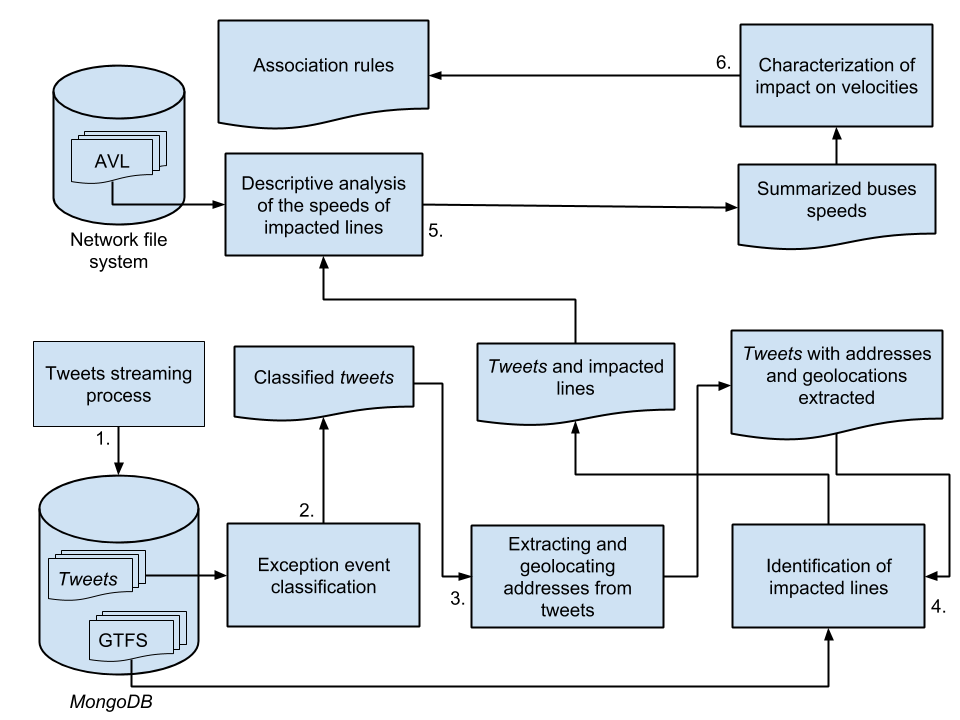
\includegraphics[width=0.5\linewidth]{caracterization_flow_en.png}
	\label{fig:caracterization_flow_en}
\end{figure}

\subsubsection{Natural Language Processing}
\label{nlp}

Before the Natural Language Processing (NLP), the \textit{tweets} were preprocessed --- removing \textit{URLs}, \textit{datetime}, mentions to other \textit{tweets}, emoticons, punctuations --- to reduce the dimension of feature space. A particular attention was paid to \textit{hashtags}, which are relevant to exception events classification, but adds noise to the address extraction phase. In order to mitigate this problem, \textit{hashtags} are identified and replaced by empty spaces in the address extraction process. Also, it is important to note that \textit{hashtags} are not removed from original \textit{tweets}.
%, involving interdisciplinary knowledge mainly among the areas of Computer Science, Linguistics and Statistics. 
%The problems related to NLP can be divided into low and high level problems.

After the preprocessing phase we applied NLP techniques to \textit{tweets}, such as (I) \textit{Tokenization} --- process to obtain the words, i.e. tokens (features used to train the classification model), in a \textit{tweet}, removing numbers and characters that do not belong to the alphabet (\textit{TweetTokenizer}\footnote{NLTK module used to the tokenization process. \url{https://www.nltk.org/api/nltk.tokenize}. Accessed in December 09, 2018.}); (II) morphological decomposition to get a given word into its inflected form using lemmatization (word lemma identification) or stemming (identification of the root of the word using heuristics to determine the location of its flexion --- \textit{RSLPStemmer}\footnote{NLTK module used to the stemming process. \url{https://www.nltk.org/\_modules/nltk/stem/rslp}. Accessed in December 09, 2018.}); process used to features space reduction, besides of Brazilian Portuguese \textit{stopwords} remotion\footnote{Brazilian Portuguese \textit{stopwords} were obtained from NLTK --- \url{https://www.nltk.org}. Accessed in December 19, 2018.} (common words without meaning) \cite{Setiawan2017, nadkarni2011natural, Korenius, roy2017understanding, collobert2011natural}.

\subsubsection{Classification model}
\label{featuresEng}

Finding exception events involves the identification of events related to an exception, which is possible through classification. Based on \cite{Itoh2016, Chen2016, Lecue2014, Gal-Tzur2014} we can use the following classes of exception events to classify the \textit{tweets}: (I) Accidents, (II) social events, (III) urban events, (IV) natural disasters and (V) irrelevant. Using the these classes, 60,984 \textit{tweets} from selected accounts were manually classified. This labeled data was transformed to a binary representation of features, which was used to train models to classify \textit{tweets} in exception events. 

%The process of constructing these features is known as \textit{feature engineering}, that is iterative between the phases of feature extraction, feature construction, and feature selection. Before this iteration, the data can be preprocessed using standardization, normalization, noise removal, dimensionality reduction, discretization, expansion, etc; it is important to note that information can be lost when performing these transformations \cite{guyon2006introduction}.

%As mentioned in Section~\ref{nlp}, we used a preprocessing phase to feature extraction through a NLP function. The feature construction and selection phases are not used because these processes do not apply to the methodology of this work. 

After the preprocessing the \textit{tweets} are processed to be represented by a bag-of-words, which contains feature vectors created using the \textit{Term Frequency - Inverse Document Frequency} (TF-IDF) measure. The bag-of-words is randomly partitioned into training (60\%) and test (40\%) sets, that are inputs to the classification algorithms.


%, however, are mentioned to a better understanding.

%In the phase of feature construction a process is performed to discover missing information regarding the relationships between features and to increase the space of features by inferring or creating new features with the objective of improving the accuracy of classification algorithms, understanding the data, obtaining hidden data, etc. At this stage, from a set of \textit {n features} $A_1, A_2, ..., A_n$ it is possible to construct additional features $A_{n+1}, A_{n+2}, ..., A_{n+m}$, by means of heuristics, logical operators, algorithms, etc \cite{motoda2002feature}.

%The feature extraction process, uses a mapping function to extract a minimal set of new features based on the original features and performance metrics, unlike the analysis of the relationships between \textit{features} performed in the \textit{feature construction} phase. Thus, with an initial set of \textit {n features} $A_1, A_2, ..., A_n$ it is possible to extract new features $B_1, B_2, ..., B_m (m <n), B_i = F_i (A_1, A_2, ..., A_n)$, where $F_i$ is the mapping function. Analogously in the \textit{tweets} processing, the features space is composed by each word (extracted from the Tokenization process), which is reduced through a stopword and stemmer functions \cite{motoda2002feature}. 

%Finally, the objective in the process of feature selection is the optimal reduction of the space of \textit {features} based on selection criteria, that is, to obtain \textit {m features} from a set of \textit{n features}, where \textit {m} $ \le $ \textit {n} (which can be achieved by search algorithms following evaluation criteria). Thus, with a smaller subset of \textit {features}, it is possible to reduce the dimensionality of the \textit {features} space, to optimize Machine Learning algorithms and to better understand their respective results, to improve the accuracy of the classification algorithms, among other benefits \cite{motoda2002feature}.

%Machine Learning algorithms can be (I) supervised, in which relations with known results are created based on the input characteristics; (II) unsupervised, in which the input characteristics are known, but not the results; (III) semi-supervised, in which some of the relationships between input data and results can be defined.
In this work we used supervised learning, since we know how the input data can be classified, being the following algorithms\footnote{We used the algorithms implemented by \textit{Sci-Kit Learn}, with the standard hyper-parameters. It is not the focus of this work hyper-parameters tuning.} normally applied to classify textual data sets: (Complement and Multinomial) Naive Bayes, Decision Tree, K-Nearest Neighbors, Logistic Regression, Multi-layer Perceptron, Random Forest and Support Vector Machine \cite{kotsiantis2007supervised, dwivedi2016automatic, narayanan2017survey}. The validation of the models to classification tasks was realized through 10-fold cross-validation\footnote{\url{https://scikit-learn.org/stable/modules/cross_validation.html\#cross-validation}. Accessed in December 26, 2018.} (to validate the generalization of a model), accuracy, precision, recall and $f_1$ score.
%\noindent
%\begin{equation*}
%Accuracy = \frac{TP + TN}{P + N} = \frac{TP + TN}{TP + TN + FP + FN}; Precision = \frac{TP}{TP + FP}
%\end{equation*}
%
%\noindent
%\begin{equation*}
%Recall = \frac{TP}{TP + FN}; F_1 score = \frac{Precision * Recall}{Precision + Recall} = \frac{2TP}{2TP + FP + FN}
%\end{equation*}

\subsubsection{Addresses and geolocalization extraction}

Analyzing the content of \textit{tweets} from the selected accounts, it is possible to observe that the texts published normally follows a given template and, therefore, are actually semi-structured. So, we used this regular expression to extract addresses from \textit{tweets}: $ER = \lbrace L_1 | S_1 | L_2 | S_2 | \dots | L_n | S_n \rbrace \lbrace [a-z\grave{A}-\ddot{y}\_] + \rbrace$.
That expression is divided in two sets, in the first ($\lbrace L_1 | S_1 | L_2 | S_2 | \dots | L_n | S_n \rbrace $), (L --- in Portuguese: \textit{logradouro}, meaning public spaces such as avenue, etc.) and (S --- public spaces acronyms) are concatenated to specify a filter and identify \textit{strings} initialized with public spaces or its respective acronyms. The second set ($\lbrace [a-z\grave{A}-\ddot{y}\_] + \rbrace $), represents a filter to identify a set of words after L or S, candidates to compose the wanted addresses.

These words are treated as candidates because it is hard to know how many words after L or S belongs to the address, however, the selected accounts publish \textit{tweets} with visible patterns in the texts, after and before the addresses. As a consequence, a possible method to find the wanted address is the removal of these patterns after and before of the address. After address extraction, we used the Google Maps Geocoding API\footnote{\url{https://developers.google.com/maps/documentation/geocoding}. Accessed in December 20, 2018.} to geolocate the found address (only 1.5\% of \textit{tweets} have geolocalization \cite{niu2016community}).
%The URL parameters utilized in this work to call the API mentioned before are: (I) \emph{address} --- the wanted address; (II) \emph{bounds} --- the bounding box which can fully contain the returned result, which one is specified by the latitude/longitude coordinates of the southwest and northeast corners of São Paulo; (III) \emph{region} --- region code with two characters i.e.: br for Brazil, and (IV) \emph{token} --- token used on API authentication.
The HTTP response from this API is processed to get the values from location (which contains latitude and longitude information) and formatted address.

%It is important to observe that the tokens from extracted address (not formatted address) are corpus-specific stop words in case of high frequency of exception events located at this address, \todo{DC: não entendi lhufas :) Se for de um evento com uma alta frequência (freq. de quê? postagens? mas isso acontece?), então o endereço é uma stop word, mas daí ele é relevante como feature?} due the fact that in this scenario they are handled as relevant features to the classification model. Therefore, the extracted address tokens are stored to be removed in \textit{tweets} processing phase.

\subsubsection{Finding bus lines affected by exception events}

In order to find the bus lines affected by exception events, it is necessary to correlate the coordinates of exception events with the existing coordinates in the shapes data set --- a set of latitude and longitude used for drawing bus lines on a map to represent its respective paths --- existing in SPTrans' GTFS. According to Section~\ref{dataSet}, all coordinates are stored in legacy pairs and in collections with geospatial indexes. Thus, it is possible to use the \texttt{\$near} function from MongoDB\footnote{\url{https://docs.mongodb.com/manual/reference/operator/query/near}. Accessed in December 18, 2018.} to find shapes close to the exception event coordinates. The GTFS defines that the \textit{shape\_id} (i.e. bus code line) is part of attributes contained in the shape file, which is used as parameter to correlate the bus code line with others GTFS files with details about the bus direction, identification, etc.

\subsubsection{Velocity impact analysis}

After we found the bus lines impacted by exception events, we select the movement data that will be analyzed, e.g. if the exception event happened on 08/17/2017 (Thursday), every other Thursday in the month of August (3, 10, 24 and 08/31/2017) will be considered in the analysis, this because the days of the week have different patterns of movement (seasonality), e.g. on Fridays many social events occur that usually lead to a more congested traffic. Besides, the months also have different characteristics --- holidays at the end of the year, vacations, beginning of school periods, etc. ---, as Fig. \ref{fig:exception_events_classification_distribution}, because of this the selected days are restricted to the month of occurrence of the event.

In another step, we also filtered the data related to the impacted lines within a radius of 100 and 1,000m of the exception event in question, in addition to considering the same time range as the \textit{tweet} time\footnote{It is important to note that this work does not consider the exact start and end of the exception events, but a time range of one hour from the time in the \textit{tweet} \textit{timestamp}.}. So, if the \textit {tweet} time is at 5:15 p.m., we considered the AVL data between 5:00 p.m. and 6:00 p.m.

Next, we aggregated the selected data to descriptively analyze the instantaneous speed of each bus line, thereby extracting data on the maximum, minimum, mean, median, variance, standard deviation and percentage of equal and non-zero data. After that, we compared the average speed of the occurrence time range with the average speed of days that do not reference the exception event, for each set of lines affected by the exception event and for each line. Finally, we considered that the line was impacted if the mean of the average speeds of the analyzed days is greater than or equal to the average speed of the day referring to the exception event. Based on this, we assumed that the set of lines has been impacted if the number of impacted lines is greater than or equal to 50\%.


\section{Results}

The methodology was applied to the \textit{Corpus Twitter}\footnote{Data set publicly available at: \url{https://github.com/fcas/mobility-analysis/blob/master/datasets/tweets.zip}. Accessed in December 14, 2018.}, which contains 60,984 \textit{tweets}. At the end of \textit{tweets} preprocessing and processing, the corpus got 414,637 words, with a vocabulary size of 13,915 words. All \textit{tweets} were manually classified according to identified exception events. This data set is composed of the following labels: Accident, Irrelevant --- to non exception events, Natural Disaster, Social Event and Urban Event.
%that distribution is illustrated in the Figure \ref{fig:pizza_events}.
 
%\begin{figure}[!htb]
%	\centering
% 	  \caption{Sentence length histogram of \textit{Corpus Tweets}}
%		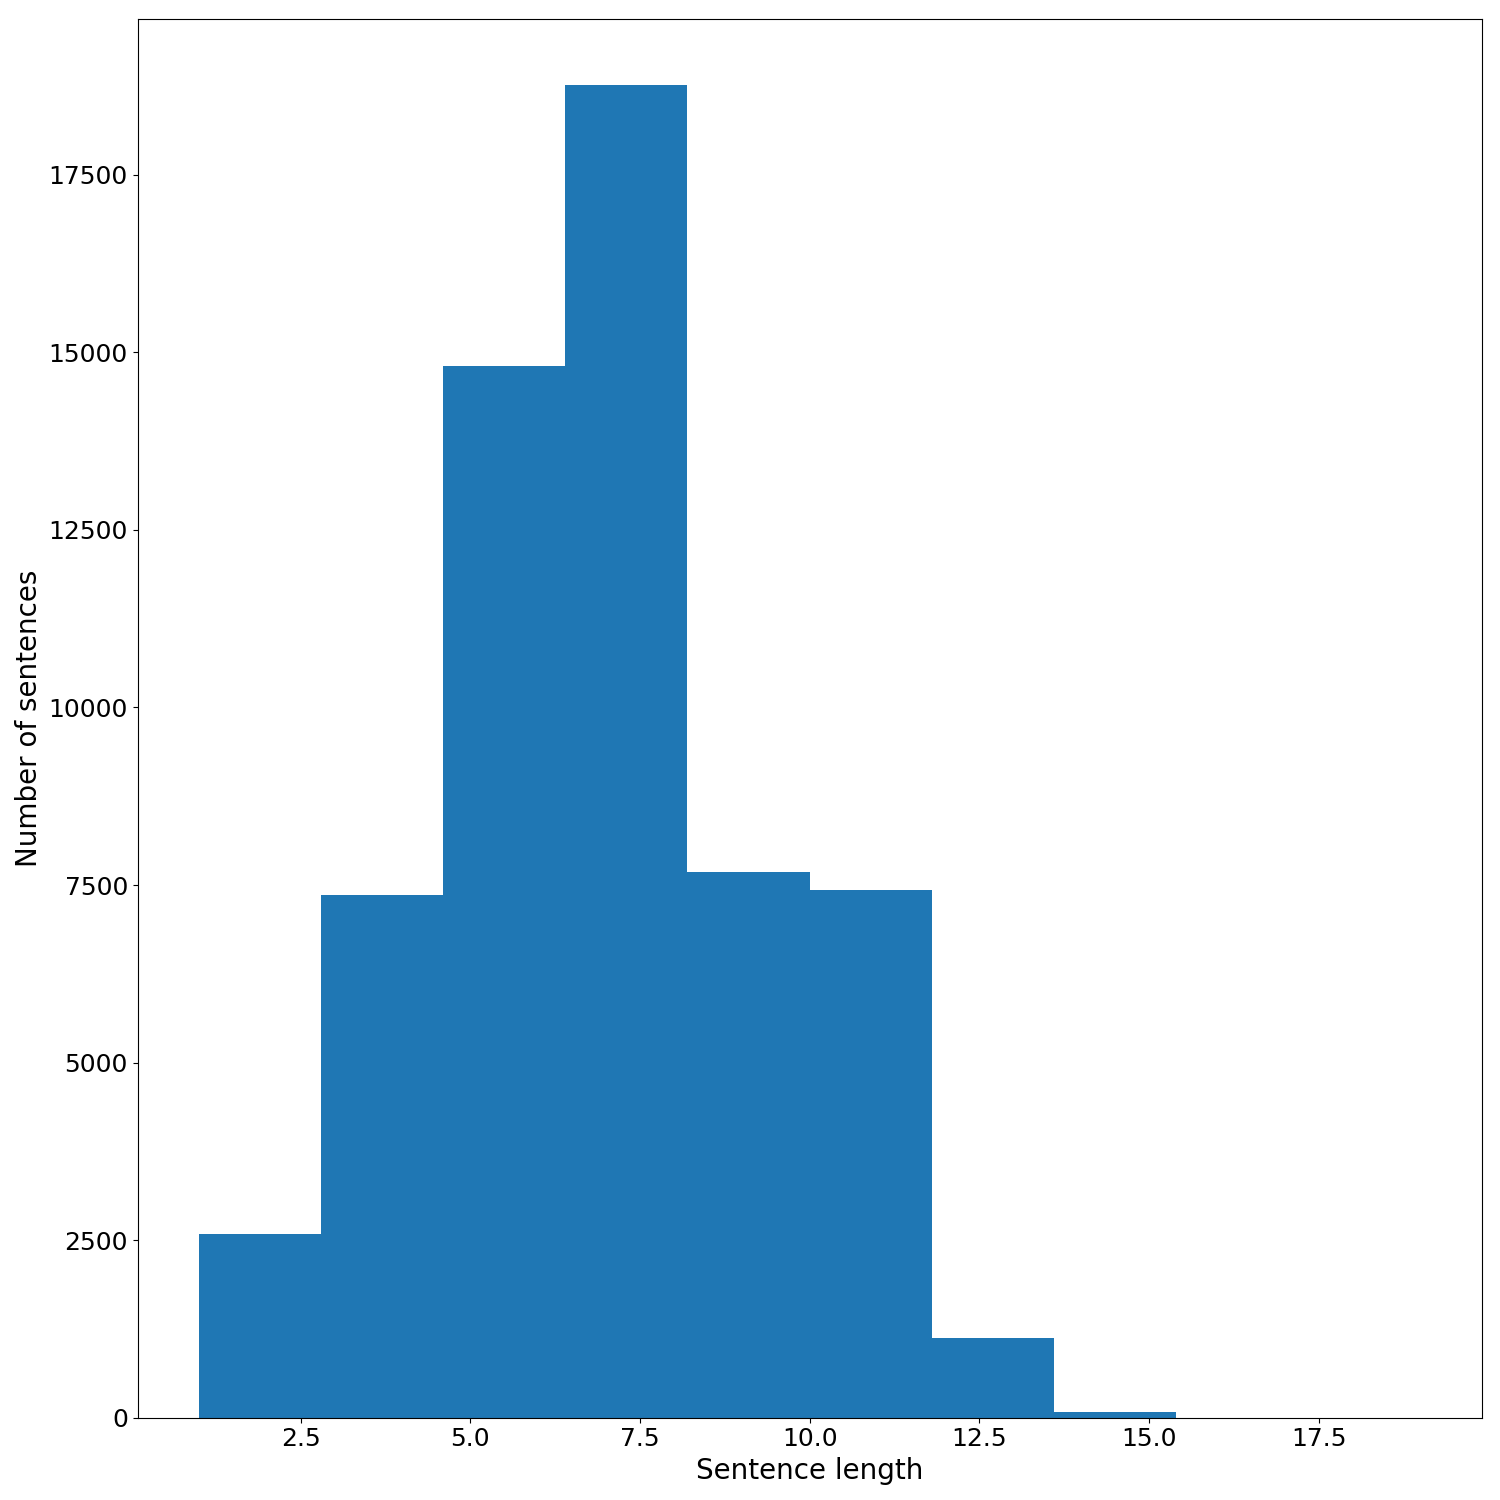
\includegraphics[width=0.7\linewidth]{corpus_metrics.png}
%	\label{fig:corpus_metrics}
%\end{figure}

%\begin{figure}[!htb]
%	\centering
% 	  \caption{Exception events distribution according to event type}
%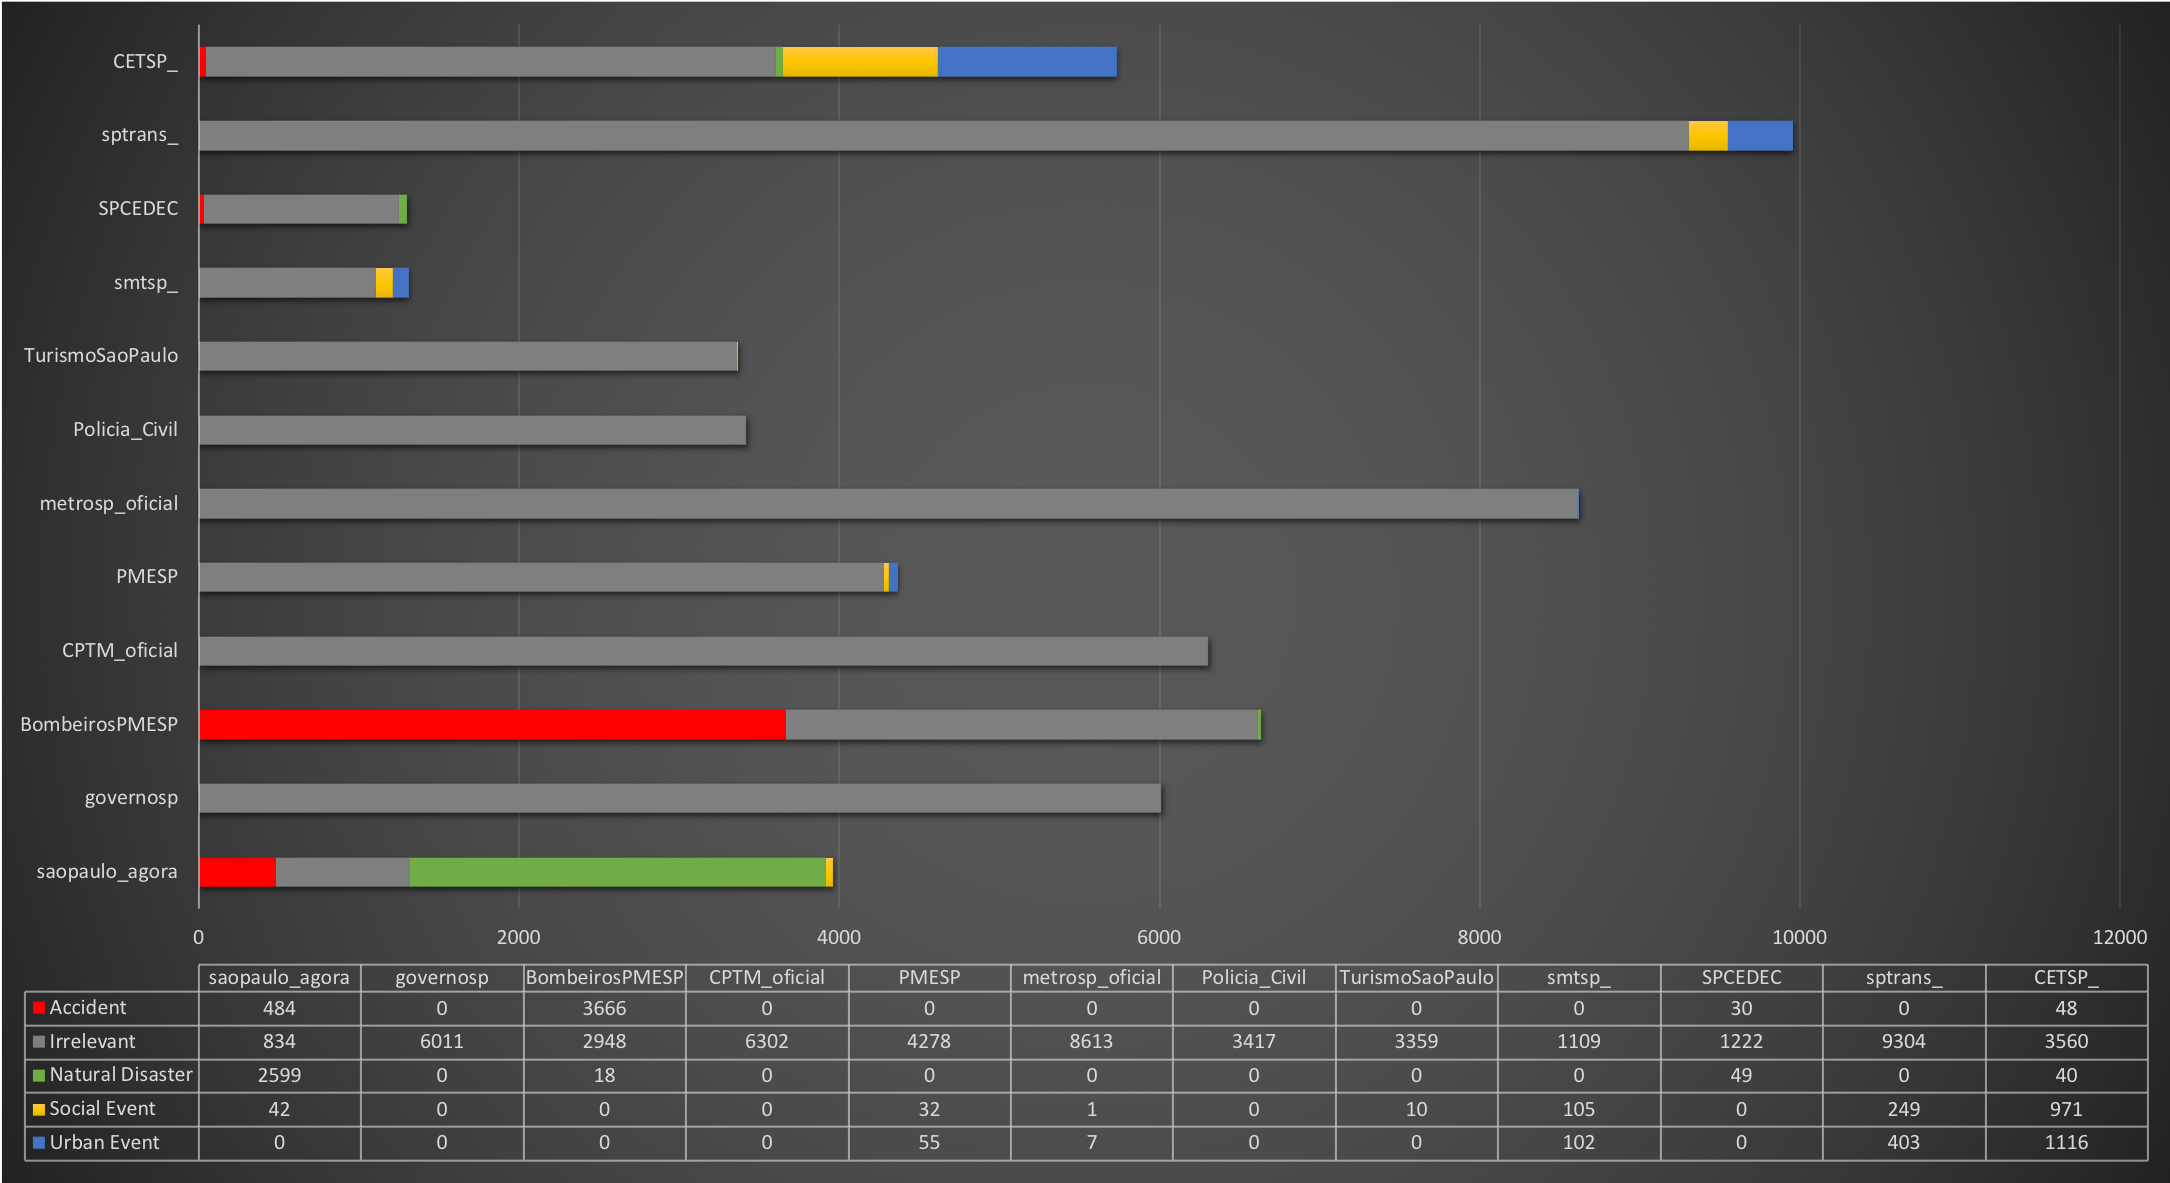
\includegraphics[width=1\linewidth]{tweets_distribution.png}
%	\label{fig:pizza_events}
%\end{figure}

This labeled data set was used to train exception events classification models, based on a \textit{bag-of-words}, described in Section~\ref{featuresEng}. According to Table~\ref{tab:metrics}, the model using the Multi-layer Perceptron algorithm obtained greater accuracy for the classification task. 

%The confusion matrix related to the Multi-layer Perceptron algorithm is illustrated by Figure ~\ref{fig:confusion_matrix_mlpc}.

\begin{table}[!htb]
\centering
\caption {Metrics of the evaluations of the algorithms used to classify the \textit {tweets} in exception events}
\label {tab:metrics}
\resizebox{8cm}{!}{
\begin{tabular}{c|c|c|c|c}
\toprule
\textbf{Algorithm} & \textbf{Accuracy} & \textbf{Precision} & \textbf{Recall} & \textbf{\textit{f1-score}} \\
\midrule
\textit{Complement Naive Bayes} & 0,941 & 0,949 & 0,941 & 0,944 \\
\hline
\textit{Decision Tree} & 0,965 & 0,965 & 0,965 & 0,965 \\
\hline
\textit{K-Nearest Neighbors} & 0,970 & 0,971 & 0,970 & 0,970 \\
\hline
\textit{Logistic Regression} & 0,969 & 0,968 & 0,969 & 0,968 \\
\hline
\textit{Multi-layer Perceptron} & \textit{0,973} & \textit{0,972} & \textit{0,973} & \textit{0,972} \\
\hline
\textit{Multinomial Naive Bayes} & 0,953 & 0,952 & 0,953 & 0,949 \\
\hline
\textit{Random Forest} & 0,970 & 0,970 & 0,970 & 0,970 \\
\hline
\textit{Support Vector Machine} & 0,833 & 0,694 & 0,833 & 0,757 \\
\bottomrule
\end{tabular}
}
\end{table}

%\begin{figure}[!htb]
%	\centering
% 	  \caption{Confusion matrix related to \textit{tweets} classification using the Multi-layer Perceptron algorithm}
%		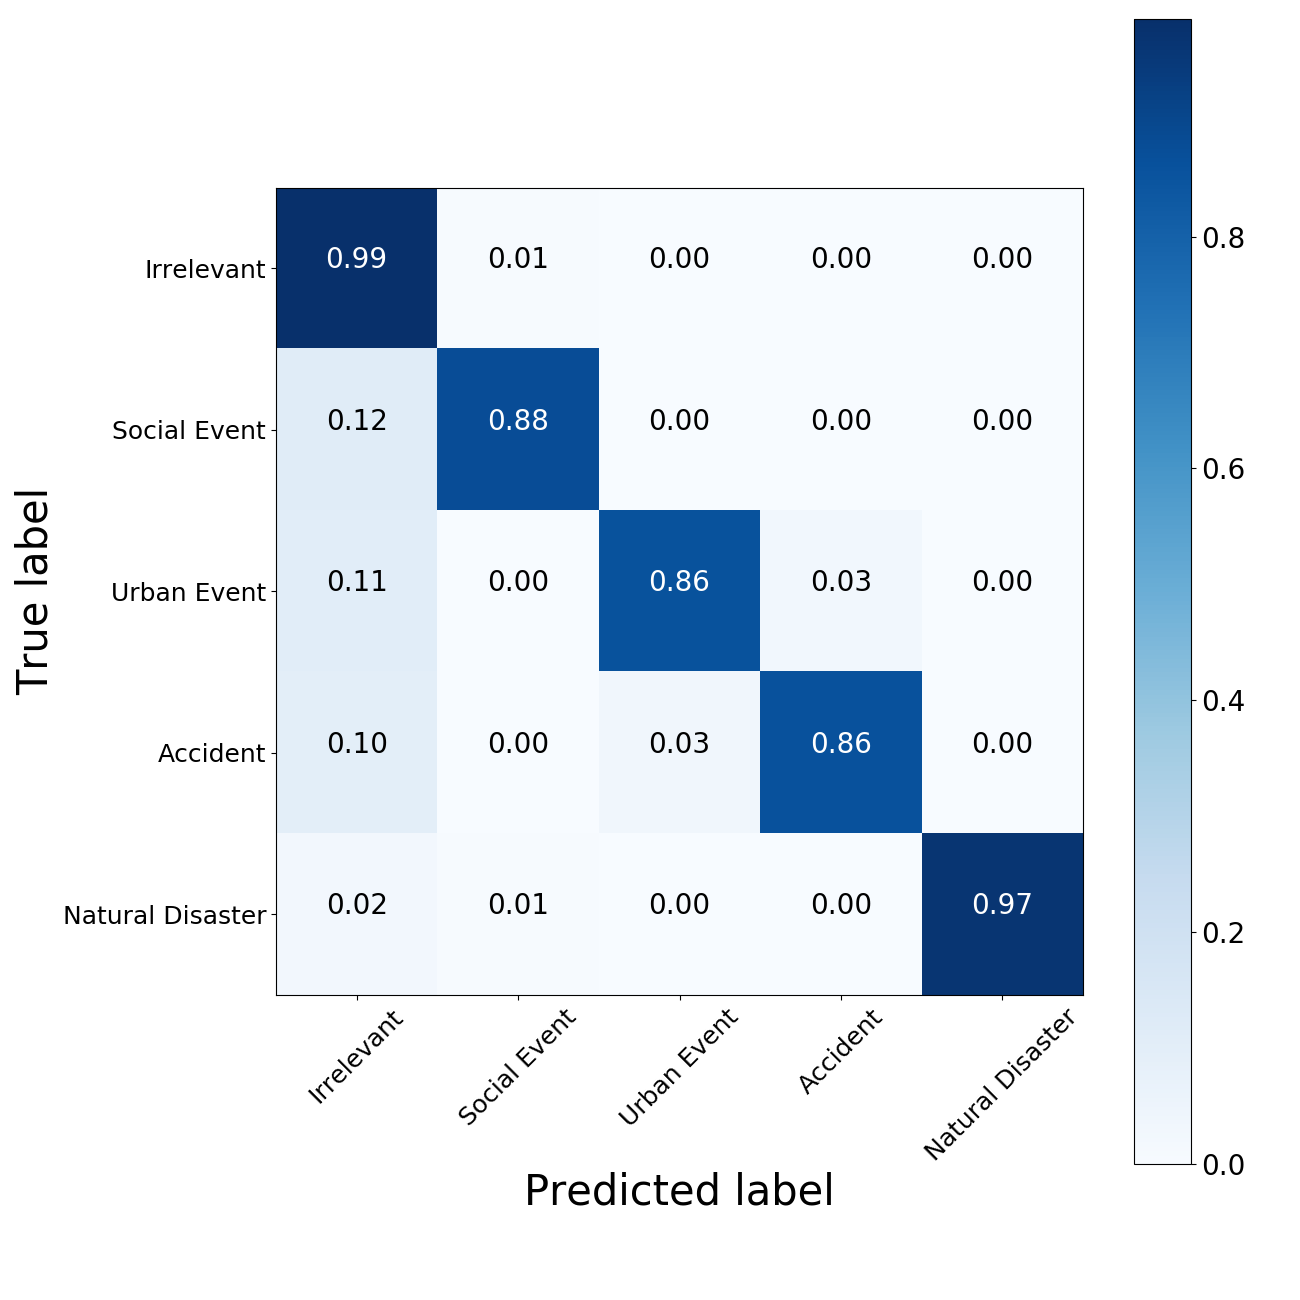
\includegraphics[width=1\linewidth]{confusion_matrix_mlp.png}
%	\label{fig:confusion_matrix_mlpc}
%\end{figure}

Of the 60,984 \textit{tweets} 10,027 were classified into exception events and from that subset we found 7,710 addresses
%, according to Tab. \ref{tab:qtdExtractedAddresses} --- disregarding the APPROXIMATE locale type\footnote{The locale type explanations can be accessed at \url{https://developers.google.com/maps/documentation/geocoding}. Accessed on December 14, 2018.} --- 
(which represents 76.89\% of the total of \textit{tweets} classified as exception events. The reasons for \textit {tweets} without address extracted are:

\begin{enumerate*}
\item \textit{Tweets} with only the point of interest, in other words, the address is not explicitly stated.
\item \textit{Tweets} without address information.
\item \textit{Tweets} with unusual public place name (for example \emph{passageway}, \emph{road complex}, \emph{connection to}).
\item \textit{Tweets} with addresses with concatenated words (for example \emph{avenidapaulista})
\end{enumerate*}

%In this case study, we disregarded the addresses with the \textit{APPROXIMATE} classification, due to the fact that they could compromise the reliability of the analyzes performed.

%\begin{table}[!htb]
%\centering
%\caption{Number of events extracted by class}
%\label {tab:qtdExtractedAddresses}
%\begin{threeparttable}
%\begin{tabular}{c|c|c|c|c|c}
%\toprule
%\textbf{Class} & \textbf{Ttl. extracted addresses} & \textbf{\textit{Ttl. APP\tnote{a}}} & \textbf{\textit{Ttl. GEO\tnote{b}}} & \textbf{\textit{Ttl. RANGE\tnote{c}}} & \textbf{\textit{Ttl. ROOF\tnote{d}}} \\
%\midrule
%Accident & 3.439 & 7 & 805 & 1.130 & 1.497 \\
%\hline
%Irrelevant & 451 & 13 & 292 & 6 & 140 \\
%\hline
%Natural Disaster & 2.464 & 9 & 340 & 719 & 1.396 \\
%\hline
%Social Event & 793 & 4 & 761 & 2 & 26 \\
%\hline
%Urban Event & 1.002 & 4 & 942 & 10 & 46 \\
%\midrule
%{} & 8.149 & 37 & 3.140 & 1.867 & 3.105 \\
%\bottomrule
%\end{tabular}
%\begin{tablenotes}
%\item Total addresses extracted with locale type
%$^a$\textit{APPROXIMATE}, $^b$\textit{GEOMETRIC\_CENTER}, $^c$\textit{RANGE\_INTERPOLATED}, $^d$\textit{ROOFTOP}.
%\end{tablenotes}
%\end{threeparttable}
%\end{table}

%The locale types\footnote {Available at \url{https://developers.google.com/maps/documentation/geocoding}. Accessed on December 14, 2018.} can be classified in:
%\begin{enumerate*}
%\item \textit {ROOFTOP} --- Indicates that the returned result has location information accurately at the street address level.
%\item \textit {RANGE\_INTERPOLATED} --- Indicates that the returned result reflects an interpolated approximation between two precise points (such as intersections). Generally, interpolated results are returned when the rooftop geocoding codes are not available for a street address.
%\item \textit {GEOMETRIC\_CENTER} --- Indicates that the returned result is the geometric center of a result.
%\item \textit {APPROXIMATE} --- Indicates that the returned result is approximate.
%\end{enumerate*}%

Figure~\ref{fig:address_analysis} illustrates the addresses\footnote{Complete list is available at https://docs.google.com/spreadsheets/d/\newline1gn1cTDifUJEPdgcU67SC45GdYHRKmIHtAfJwRBm088s/edit?usp=sharing. Accessed on December 20, 2018.} most affected by exception events and Figure~\ref{fig:dispersion} shows the distribution of these events in the central region of São Paulo. It is important to note that the exception events found are concentrated in the addresses and regions where they normally occur in São Paulo, which validates the methodology developed.

\begin{figure}
\centering
\begin{minipage}{.5\textwidth}
  \centering
    \caption{Addresses most impacted by exception events}
    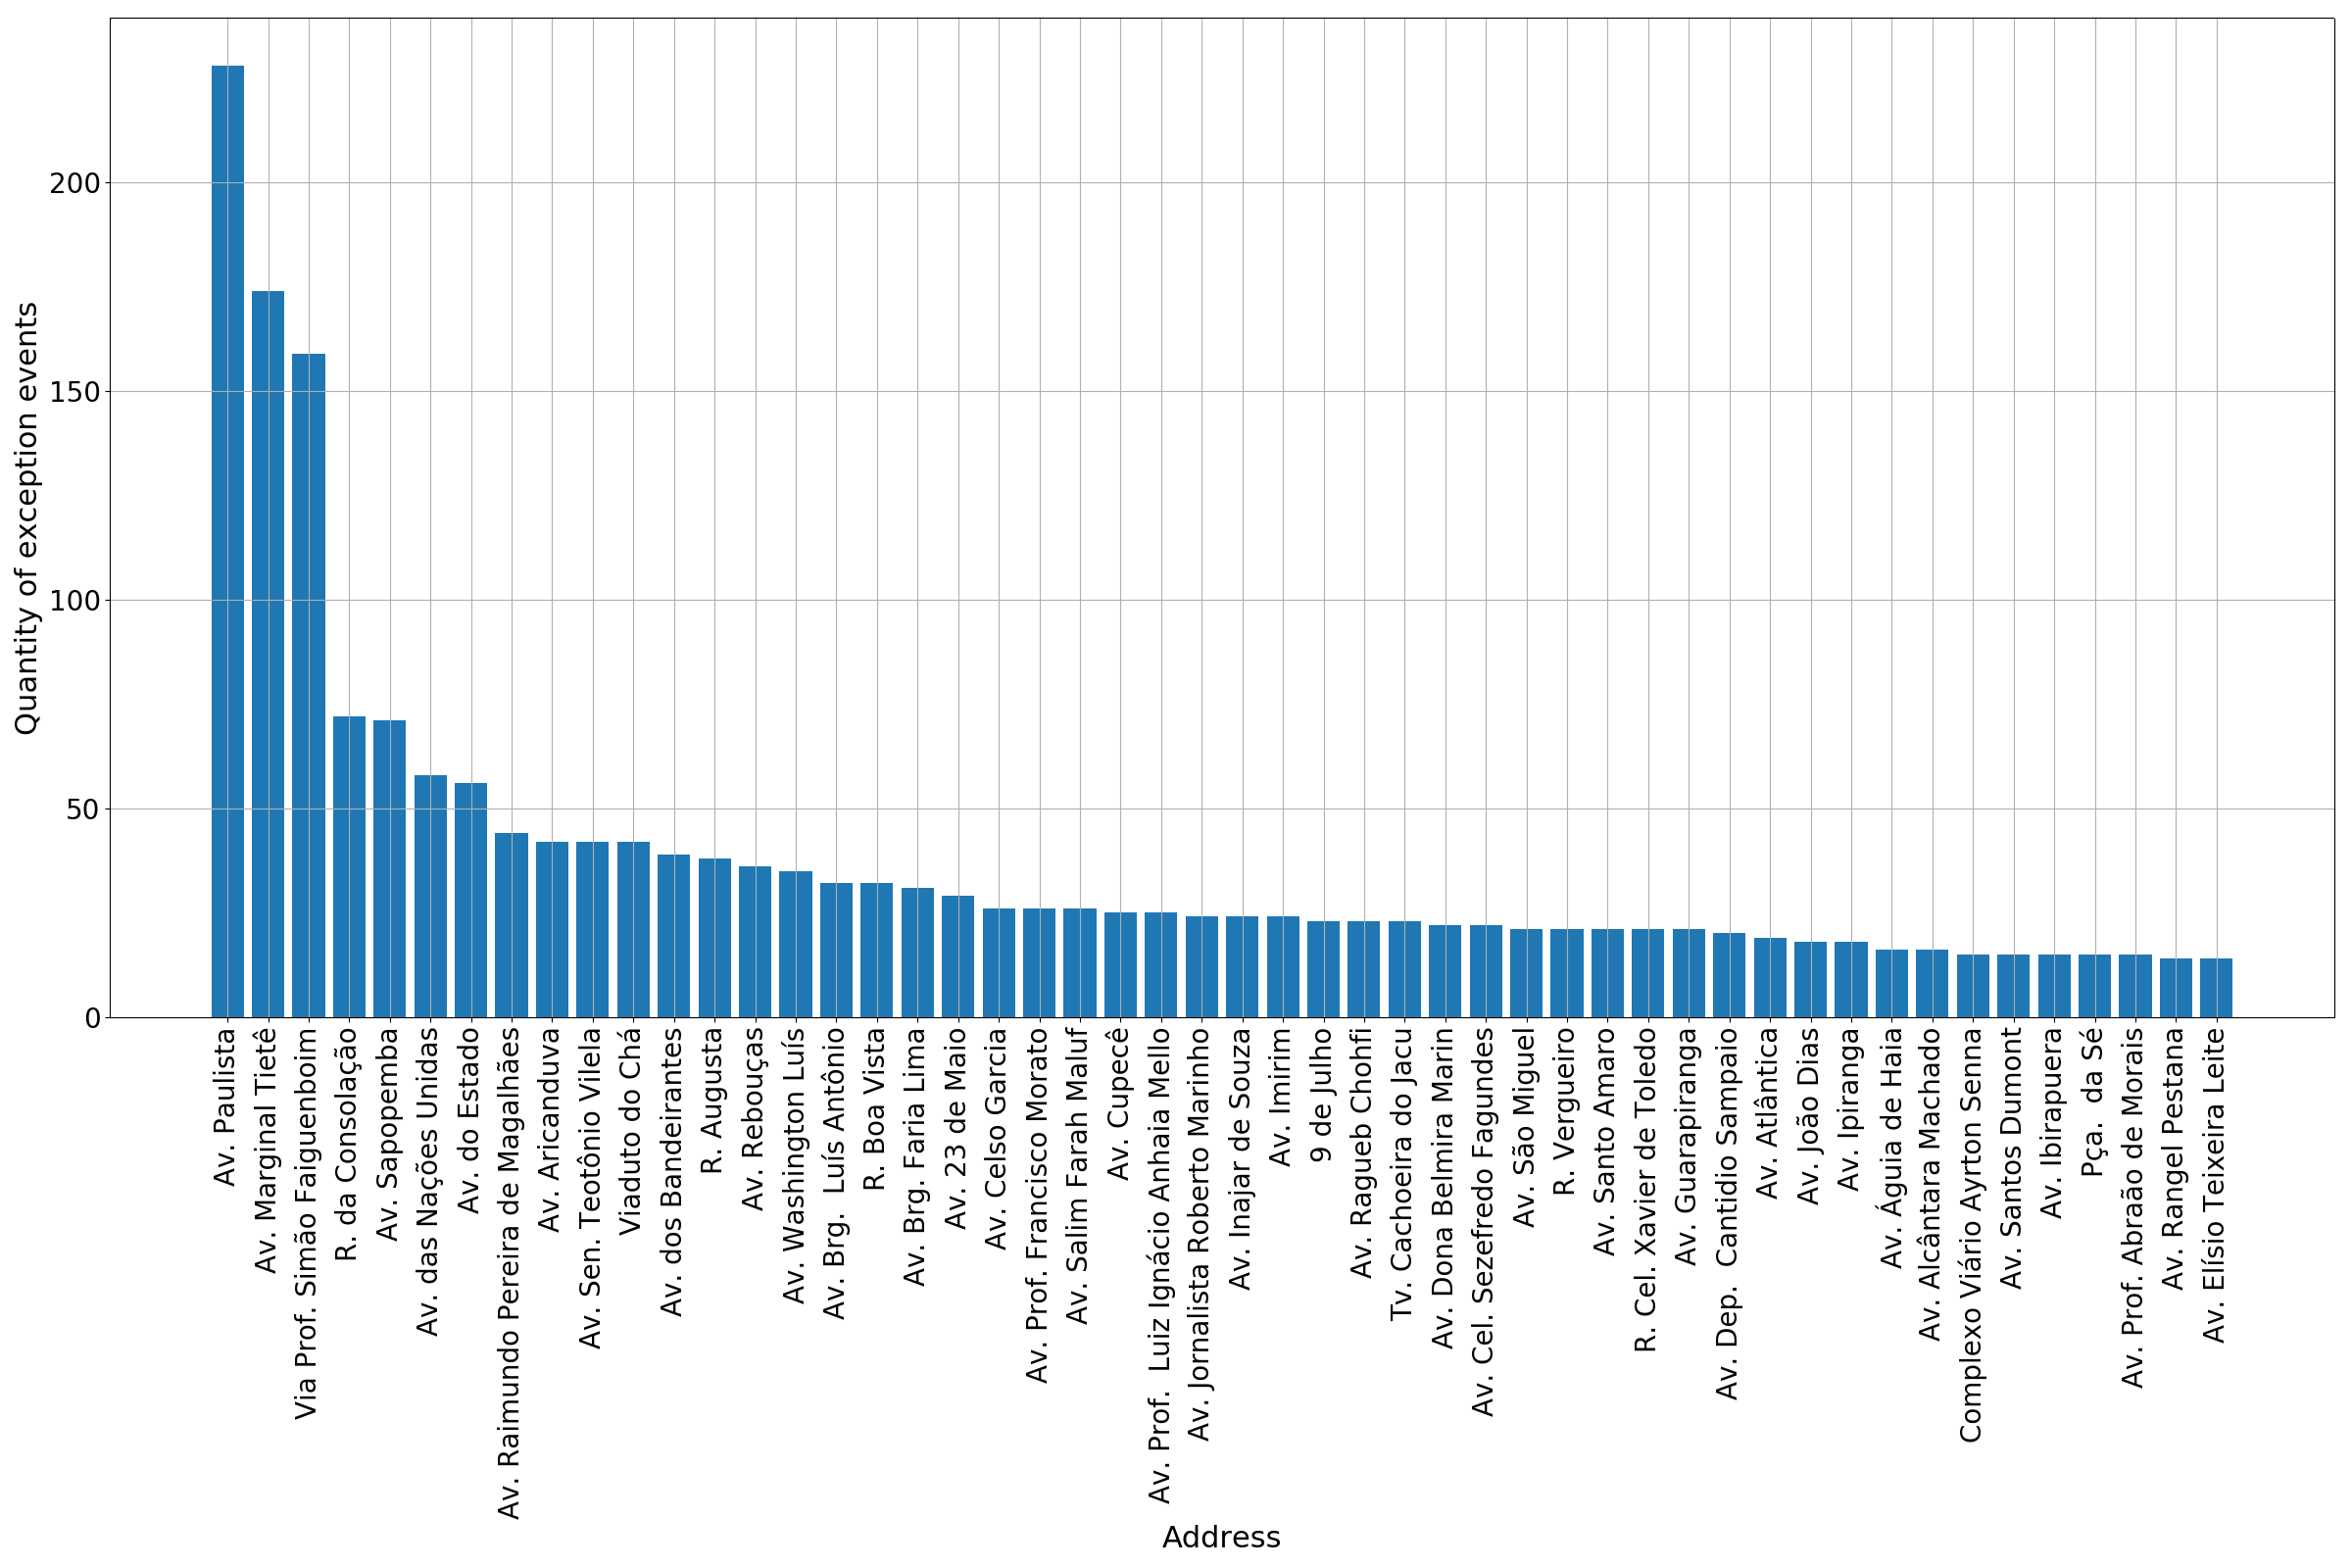
\includegraphics[width=1\linewidth]{address_analysis.png}
  \label{fig:address_analysis}
\end{minipage}%
\begin{minipage}{.5\textwidth}
  \centering
    \caption{Distribution of exception events in the central region of São Paulo}
    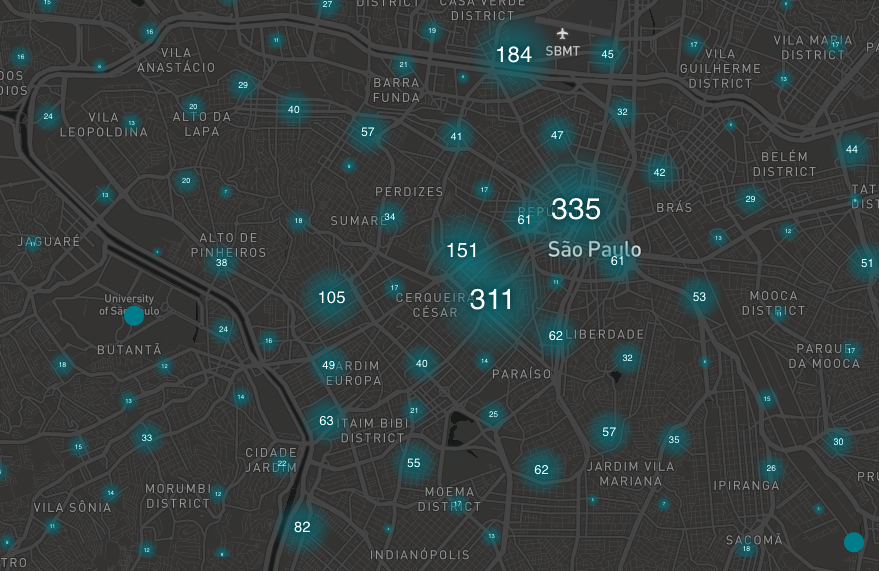
\includegraphics[width=1\linewidth]{exception_events_sp.png}
  \label{fig:dispersion}
\end{minipage}
\end{figure}

We considered that a bus line is affected by an exception event if a coordinate from \textit{shape} is within a radius of 1,000m away from the event. Using this criterion, the total of 1,073 bus lines were affected by exception events during this period, with line ``33121'' (TERM. PRINC. ISABEL / TERM. STO. AMARO) being the most impacted bus line code. This particular line was impacted by 1,623 exception events and the full table publicly available in \footnote{\url{https://docs.google.com/spreadsheets/d/1jIqUuIJg7FhXD5C8MFF8stbvOD3uiUgMfN2bOltT7zE/edit?usp=sharing}. Accessed in December 20, 2018.}.

%\begin {table} [!htb]
%\centering
%\resizebox{14cm}{!}{
%\begin{threeparttable}
%\caption {Bus lines most impacted by exception events\tnote{a}}
%\label {tab:impacted_bus_code_lines}
%\begin {tabular} {c|c|c}
% \toprule
%\textbf{Bus code line} & \textbf{Ttl. excepetion events} & \textbf{Bus origin / destination} \\
%    \midrule
%33121 & 	1623 & TERM. PRINC. ISABEL / TERM. STO. AMARO \\
%\hline
%32826 &     1502 & 	TERM. PQ. D. PEDRO II / TERM. JOÃO DIAS \\
%\hline
%32805 & 	1490 & 	TERM. PRINC. ISABEL / CHÁC. SANTANA \\
%\hline
%34085 & 	1464 & 	TERM. BANDEIRA / JD. VAZ DE LIMA \\
%\hline
%34233 & 	1418 & 	TERM. BANDEIRA / TERM. VARGINHA \\
%\hline
%33123 & 	1408 & 	TERM. BANDEIRA / TERM. STO. AMARO \\
%\hline
%32829 & 	1405 & 	TERM. BANDEIRA / TERM. CAPELINHA \\
%\hline
%35174 & 	1388 & 	TERM. PQ. D. PEDRO II / TERM. STO. AMARO \\
%\hline
%32827 & 	1378 & 	TERM. BANDEIRA / TERM. CAPELINHA \\
%\hline
%33128 & 	1373 & 	TERM. BANDEIRA / SOCORRO \\
%\bottomrule
%\end{tabular}
%\begin{tablenotes}
%            \item[a] Full table publicly available at \url{https://docs.google.com/spreadsheets/d/1jIqUuIJg7FhXD5C8MFF8stbvOD3uiUgMfN2bOltT7zE/edit?usp=sharing}. Accessed in December 20, 2018.
%        \end{tablenotes}
%\end{threeparttable}
%}
%\end{table}

\begin{table}[!htb]
\centering
\caption {Percentage of impact on the average speed of the groups of lines affected by exception events at 1,000m and 100m distance respectively, in the months of 2017}
\label {tab:exceptEventVelocityImpAll}
\resizebox{8cm}{!}{
\begin{tabular}{c|cc|cc|cc|cc}
\toprule
\textbf{Month} & \multicolumn{2}{c}{\textit{\textbf{Accident}}} & \multicolumn{2}{c}{\textit{\textbf{Natural Disaster}}} & \multicolumn{2}{c}{\textit{\textbf{Social Event}}} &
\multicolumn{2}{c}{\textit{\textbf{Urban Event}}}\\
\midrule
January & 83,33 &  100 & 
64,23 &  98,00 & 
100 & --- &
 100 & --- \\
\hline
February & 70,58 &  100 &
 66,25 &  100 &
 100 & 100 &
 80 & --- \\
\hline
March &  50,00 &  --- & 
66,66 &  100 &
85,00 & 100 &
68,18 & 100 \\
\hline
April & 87,50 &100 & 
 61,11 & 100 & 
 82,75 & 100 & 
 76,92 &  100 \\
\hline
May & 65,13 &  100 &
 58,82 &  100 &
 93,33 & 100 &
 50,00 & 100 \\
\hline
June & 54,46 &  100 &
 61,53 &  100 &
 76,47 & 100 &
 72,41 & 100 \\
\hline
July & 61,48 &  98,41 &
 66,66 & 100 &
 69,23 & 100 &
58,13 & 100 \\
\hline
August & 57,86 & 87,17 &
 55,35 & 100 &
 85,54 & 100 & 
 68,10 & 90,90 \\
\hline
September & 64,21 & 100 &
 42,10 & 100 &
 92,30 & 100 & 
 62,06 & 100 \\
\hline
October & 70,49 & --- &
 56,81 & --- &
 80,00 & --- &
 61,11 & --- \\
\hline
November & 66,66 & 100 &
 57,99 & 100 &
 92,85 & 100 &
 74,35 & 100 \\
\hline
December & --- & --- & --- & --- & --- & --- & --- & ---  \\
\midrule
\textbf{Total} & 66,51 & 98,39 & 59,77 & 99,80 & 87,04 & 100 & 70,11 & 98,86  \\
\bottomrule
\end{tabular}
}
\end{table}

\begin{figure}[!htb]
	\centering
 	  \caption{Distribution of geolocation exception classes over the months of 2017}
		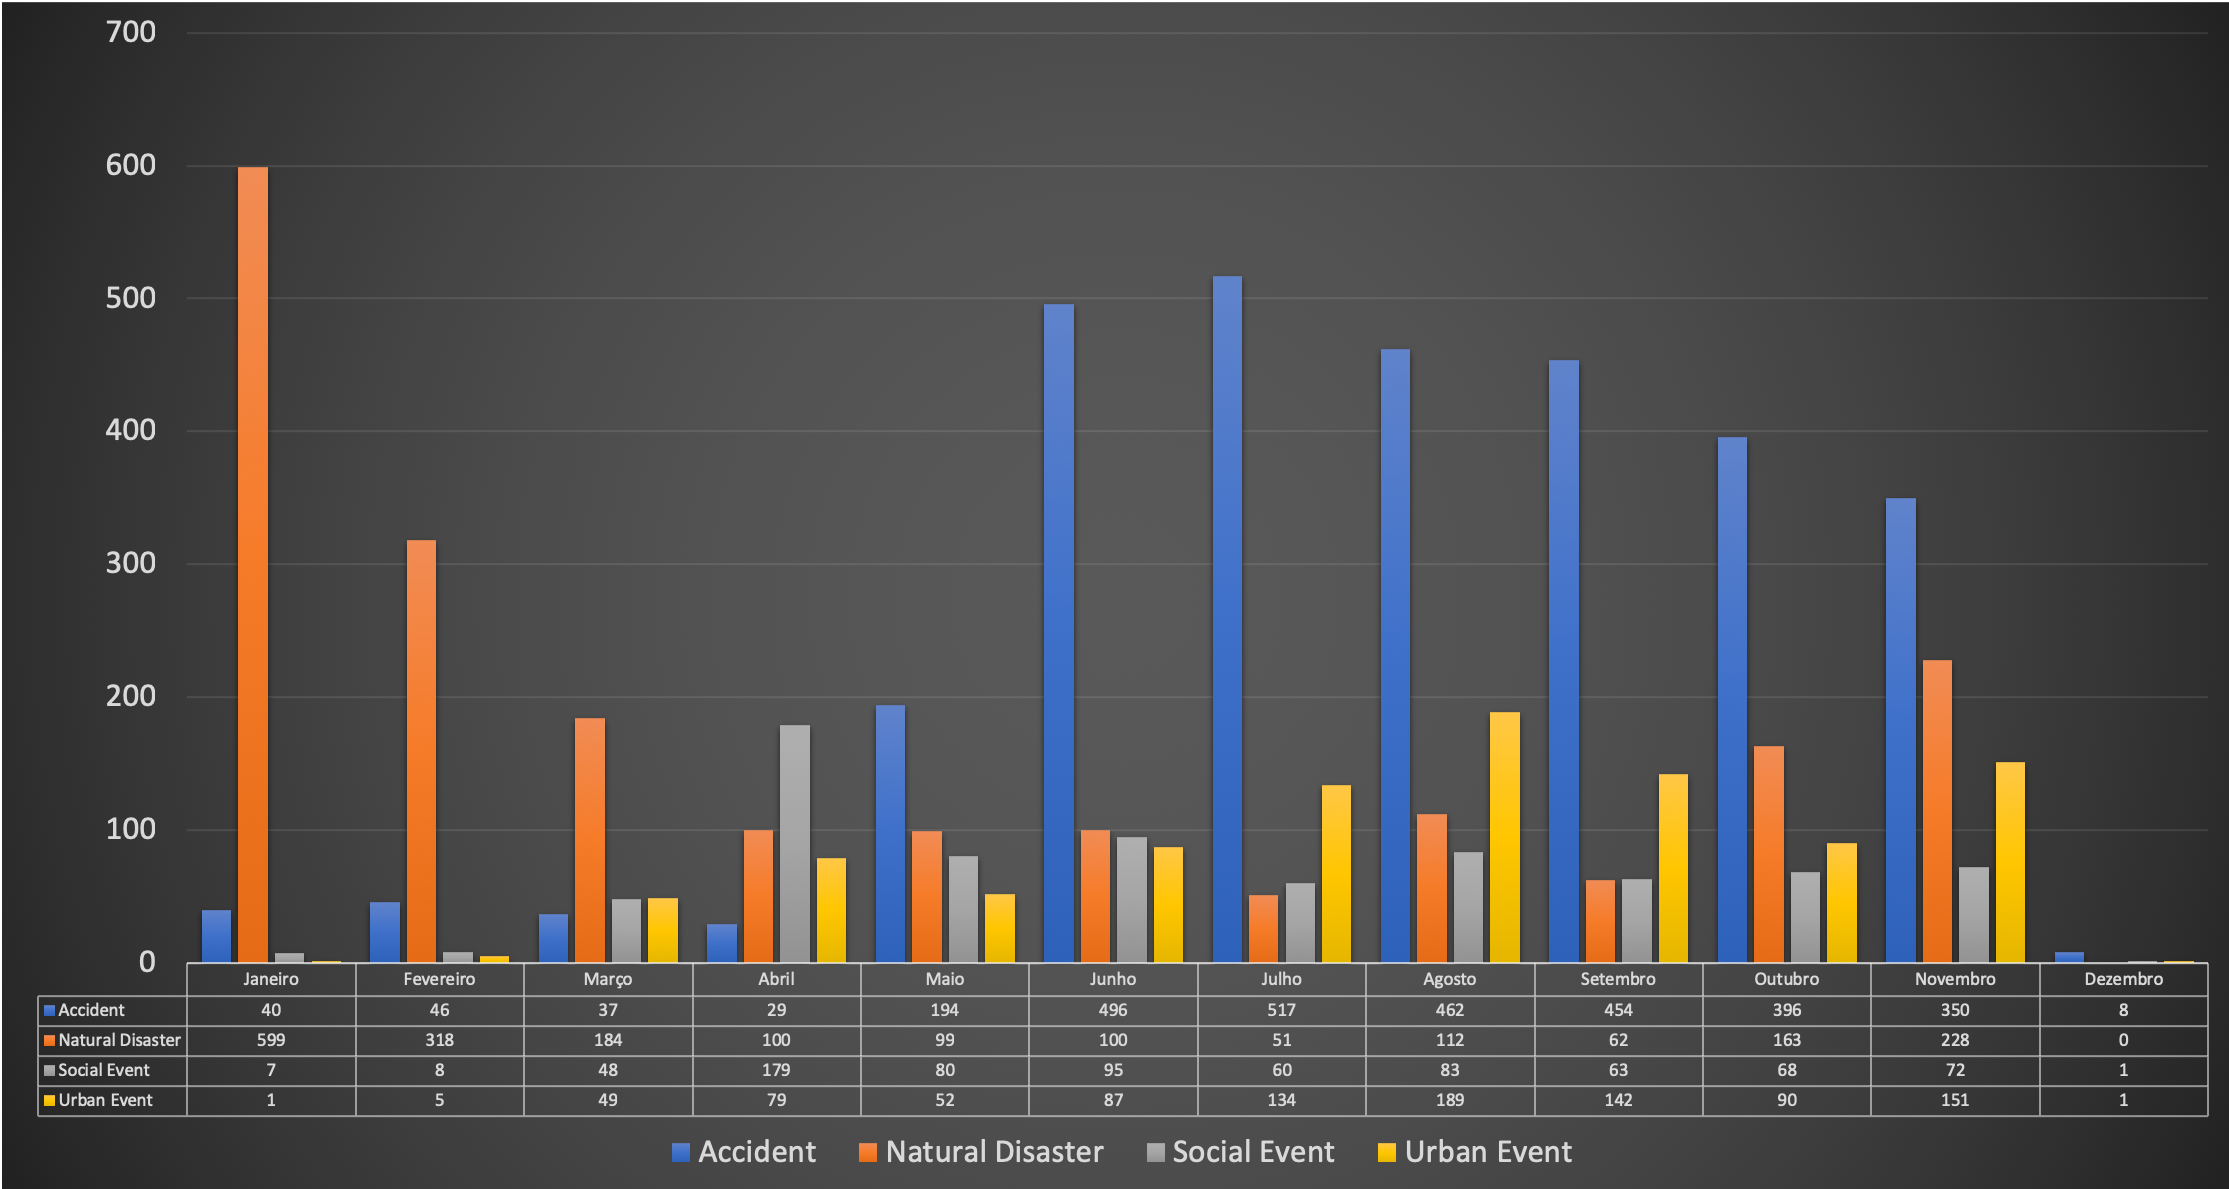
\includegraphics[width=0.7\linewidth]{exception_events_classification_distribution.png}
	\label{fig:exception_events_classification_distribution}
\end{figure}

Using the methodology described above, we can observe in Tab. \ref{tab:exceptEventVelocityImpAll} that the social event-related exception events have an average of 87,04\% impact on the average speed in the groups of bus lines affected by a radius of 1,000m and 100\% to a radius of 100m, this probably due to the large number of people involved in this type of event, number of avenues with modified or interrupted traffic flow.

Urban events, in turn, impacts 70,11\% at 1,000m and 98,86\% at 100m, even though these events are being carried out with alternative routes planning and warn signs on public roads. The third and fourth most affected classes are those of accidents and natural disasters, respectively, 66,51\% and 59,77 \% at 1,000m and 98,39 \% and 99,80 \% to 100m, which normally blockages or detours on public roads used by buses.

In addition, January, February and March were the three months most affected by exception events related to natural disasters, a period of high rainfall in São Paulo, where landslides, tree falls and floods usually occurs. In relation to social events, the year 2017 was marked with numerous political manifestations, in this context, May was the most impacted month by this type of exception event, mainly due to the protests against the government Temer \footnote{{www1.folha.uol.com.br/poder/2017/05/1884977-manifestacao-anti-\newline temer-reune-hundreds-of-people-in-av-paulista.shtml}. Accessed on December 2, 2018}. The events related to accidents usually occur in greater concentration in the periods of holidays and holidays, which can be observed in the months of January and April (single month of 2017 with two prolonged holidays), with a mean impact of 83.33\% and 87.50\% at the average speeds, respectively. Impacts related to urban events occurs normally during all months, due to which they percentages are uniform.

The months close to 100\% of impact at average speeds are justified because of the small volume of events for a given class in a given month, as Fig.\ref{fig:exception_events_classification_distribution}, which also happens for scenarios with geolocated data next to the exception events. Similarly, the months and classes without impact data are months with little data for the analyzed class.

%\begin{table}[!htb]
%\centering
%\begin{threeparttable}
%\caption {Apriori analysis applied to the average speed values (5-minute intervals) to the AVL data set of SPTrans correlated to the exception events (from distance of 100m\tnote{d} and 1,000m\tnote{e}, respectively) from the months of the year 2017}
%\label {tab:aprioriFull}
%\begin{tabular}{c|c|c|c|c|c}
%\toprule
%\textbf{\textit{Event type}} & \textbf{\textit{Total events}} & \textit{\textbf{Total rules}} & \textbf{\textit{Expected}}\tnote{a} & \textbf{\textit{Unexpected}}\tnote{b} & \textbf{\textit{P. unexpected}}\tnote{c}   \\
%\midrule
%\textit{Accident} & 1.677 & 315.063 & 278.493 & 30.804 & 5.766 \\
%\hline
%\textit{Natural Disaster} & 912 & 115.301 & 99.206 & 14.282 & 1.813 \\
%\hline
%\textit{Social Event} & 506 & 61.927 & 52.403 & 8.245 & 1.279 \\
%\hline
%\textit{Urban Event} & 596 & 93.513 & 81.261 & 10.480 & 1.772 \\
%\midrule
%{---} & 3.691 & 585.804 & 511.363 & 63.811 & 10.603 \\
%\bottomrule
%\toprule
%\textbf{\textit{Event type}} & \textbf{\textit{Total events}} & %\textit{\textbf{Total rules}} & \textbf{\textit{Expected}}\tnote{a} & %\textbf{\textit{Unexpected}}\tnote{b} & \textbf{\textit{P. unexpected}}\tnote{c}   %\\
%\midrule
%\textit{Accident} & 3.029 & 3.980.542 & 3.415.780 & 385.728 & 179.034 \\
%\textit{Natural Disaster} & 2.016 & 2.624.415 & 2.253.123 & 259.285 & 112.007 \\
%\textit{Social Event} & 764 & 1.262.805 & 1.118.546 & 100.224 & 44.035 \\
%\textit{Urban Event} & 980 & 1.481.040 & 1.296.476 & 125.803 & 58.761 \\
%\midrule
%{---} & 6.789 & 9.348.802 & 8.083.925 & 871.040 & 393.837 \\
%\bottomrule
%\end{tabular}
%\begin{tablenotes}
%            \item[a] Regradas experadas ($Lift > 1$, $Support > 0,05$)
%            \item[b] Regras inesperadas ($Lift = 1$)
%            \item[c] Regras parcialmente inesperadas ($0 < Lift < 1$)
%            \item[d] 3.545 eventos de exceção não atingiram linhas de ônibus no %raio de 100m.
%            \item[e] 447 eventos de exceção não atingiram linhas de ônibus no raio de 1.000m.
%        \end{tablenotes}
%\end{threeparttable}
%\end{table}

\section{Conclusions and future works}

This work presents a new methodology for exception events classification and analyze their respective impacts on velocity of the public transport system by bus of the São Paulo city. Using \textit{tweets} from selected public service providers, we found that Multi-layer Perceptron was the best algorithm for classifying \textit{tweets} in exception events. We also showed that it is possible to extract addresses from semi-structured \textit{tweets} using only regular expressions. Classifying these events are the first step to better understand how these exceptional events impact the velocity of buses, using the methodology developed we found that social events reduces the velocity of 87,04\% of a group impacted, urban event 70,11\%, accident 66,51\% and natural disaster 59,77\% from a distance of 1,000m.

Although validated using selected Twitter profiles written in Brazilian Portuguese language, this method can be generalized for different languages and cities. GTFS is a ubiquitous format for public transport and tools like NLTK supports several languages.

\textbf{Future work}


\section*{Acknowledgment}
This research is part of the INCT of the Future Internet for Smart Cities funded by CNPq proc. 465446/2014-0, Coordenação de Aperfeiçoamento de Pessoal de Nível Superior -- Brasil (CAPES) -- Finance Code 001, FAPESP proc. 14/50937-1, and FAPESP proc. 15/24485-9.

\bibliographystyle{splncs04}
\bibliography{references}

\end{document}
